\begin{appendix}

\chapter{Scenario Materials}
\hypertarget{tbl:zms-analysis}{}
\begin{table}[h]
  \caption{ZMS Scenario Application Quantitative Analysis Results}
  \label{tbl:zms-analysis}
  \centering
    \begin{tabularx}{0.98\linewidth}{ XX } 
    \toprule
    \textbf{Criterion} & \textbf{Number} \\
    \midrule
    directories & 31\\
    source files & 603\\
    LOC & 131,505\\
    SLOC & 106,469\\
    comment lines & 14,340\\
    mean LOC per source file & 218\\ 
    mean SLOC per source file & 177\\
    header files & 234\\
    mean header LOC & 69\\
    implementation files & 198\\
    mean implementation LOC & 398\\
    classes & 211\\
    mean methods per class & 16\\
    functions & 3362\\
    \bottomrule
    \end{tabularx}
\end{table}

\chapter{Problem Analysis Materials}
\hypertarget{tbl:stakeholders}{}
\begin{longtable}[]{@{}llll@{}}
\caption{\label{tbl:stakeholders}Stakeholder Map}\tabularnewline
\toprule
\begin{minipage}[b]{0.16\columnwidth}\raggedright
Stakeholder\strut
\end{minipage} & \begin{minipage}[b]{0.24\columnwidth}\raggedright
Interest/how affected\strut
\end{minipage} & \begin{minipage}[b]{0.24\columnwidth}\raggedright
Capacity \& Motivation\strut
\end{minipage} & \begin{minipage}[b]{0.24\columnwidth}\raggedright
Possible Actions to Address Stakeholders\strut
\end{minipage}\tabularnewline
\midrule
\endfirsthead
\toprule
\begin{minipage}[b]{0.16\columnwidth}\raggedright
Stakeholder\strut
\end{minipage} & \begin{minipage}[b]{0.24\columnwidth}\raggedright
Interest/how affected\strut
\end{minipage} & \begin{minipage}[b]{0.24\columnwidth}\raggedright
Capacity \& Motivation\strut
\end{minipage} & \begin{minipage}[b]{0.24\columnwidth}\raggedright
Possible Actions to Address Stakeholders\strut
\end{minipage}\tabularnewline
\midrule
\endhead
\begin{minipage}[t]{0.16\columnwidth}\raggedright
Software/ Migration Engineers\strut
\end{minipage} & \begin{minipage}[t]{0.24\columnwidth}\raggedright
- new knowledge\\
- increased workload through migration\strut
\end{minipage} & \begin{minipage}[t]{0.24\columnwidth}\raggedright
- key role, defining available expertise and requirements for migration activities- limited motivation improvement of product and lower effort for updates and maintenance\strut
\end{minipage} & \begin{minipage}[t]{0.24\columnwidth}\raggedright
- presentation of technology demonstrators etc.\\
- reduce workload through tailored and integrated migration methods and tools\strut
\end{minipage}\tabularnewline
\begin{minipage}[t]{0.16\columnwidth}\raggedright
Managers\strut
\end{minipage} & \begin{minipage}[t]{0.24\columnwidth}\raggedright
- higher sales\\
- reduced costs for software distribution and maintenance\\
- increased risk and workload through migration\strut
\end{minipage} & \begin{minipage}[t]{0.24\columnwidth}\raggedright
- decision taker role\\
- higher competitiveness due to improved product portfolio and reduced effort\strut
\end{minipage} & \begin{minipage}[t]{0.24\columnwidth}\raggedright
- \gls{risk management}\\
- communicate benefits through prototypes\strut
\end{minipage}\tabularnewline
\begin{minipage}[t]{0.16\columnwidth}\raggedright
Doctor's Offices\strut
\end{minipage} & \begin{minipage}[t]{0.24\columnwidth}\raggedright
- innovative features \& improved usability\\
- changes in existing work patterns- training effort- new hardware\\
- security and data privacy\strut
\end{minipage} & \begin{minipage}[t]{0.24\columnwidth}\raggedright
- customers\\
- almost no intrinsic motivation\strut
\end{minipage} & \begin{minipage}[t]{0.24\columnwidth}\raggedright
- user training\strut
\end{minipage}\tabularnewline
\begin{minipage}[t]{0.16\columnwidth}\raggedright
Patients\strut
\end{minipage} & \begin{minipage}[t]{0.24\columnwidth}\raggedright
- innovative features \& improved usability- more interactivity\strut
\end{minipage} & \begin{minipage}[t]{0.24\columnwidth}\raggedright
- customers of customers\strut
\end{minipage} & \begin{minipage}[t]{0.24\columnwidth}\raggedright
- information about new features\strut
\end{minipage}\tabularnewline
\begin{minipage}[t]{0.16\columnwidth}\raggedright
Competitors\strut
\end{minipage} & \begin{minipage}[t]{0.24\columnwidth}\raggedright
- idea transfer to own products\\
- competitive disadvantage\strut
\end{minipage} & \begin{minipage}[t]{0.24\columnwidth}\raggedright
- market share\strut
\end{minipage} & \begin{minipage}[t]{0.24\columnwidth}\raggedright
N/A\strut
\end{minipage}\tabularnewline
\begin{minipage}[t]{0.16\columnwidth}\raggedright
Companies with similar situation\strut
\end{minipage} & \begin{minipage}[t]{0.24\columnwidth}\raggedright
- solution\strut
\end{minipage} & \begin{minipage}[t]{0.24\columnwidth}\raggedright
- improved situation\strut
\end{minipage} & \begin{minipage}[t]{0.24\columnwidth}\raggedright
- dissemination of Results\strut
\end{minipage}\tabularnewline
\bottomrule
\end{longtable}

\begin{sidewaysfigure}
\hypertarget{fig:problem-tree}{%
\centering
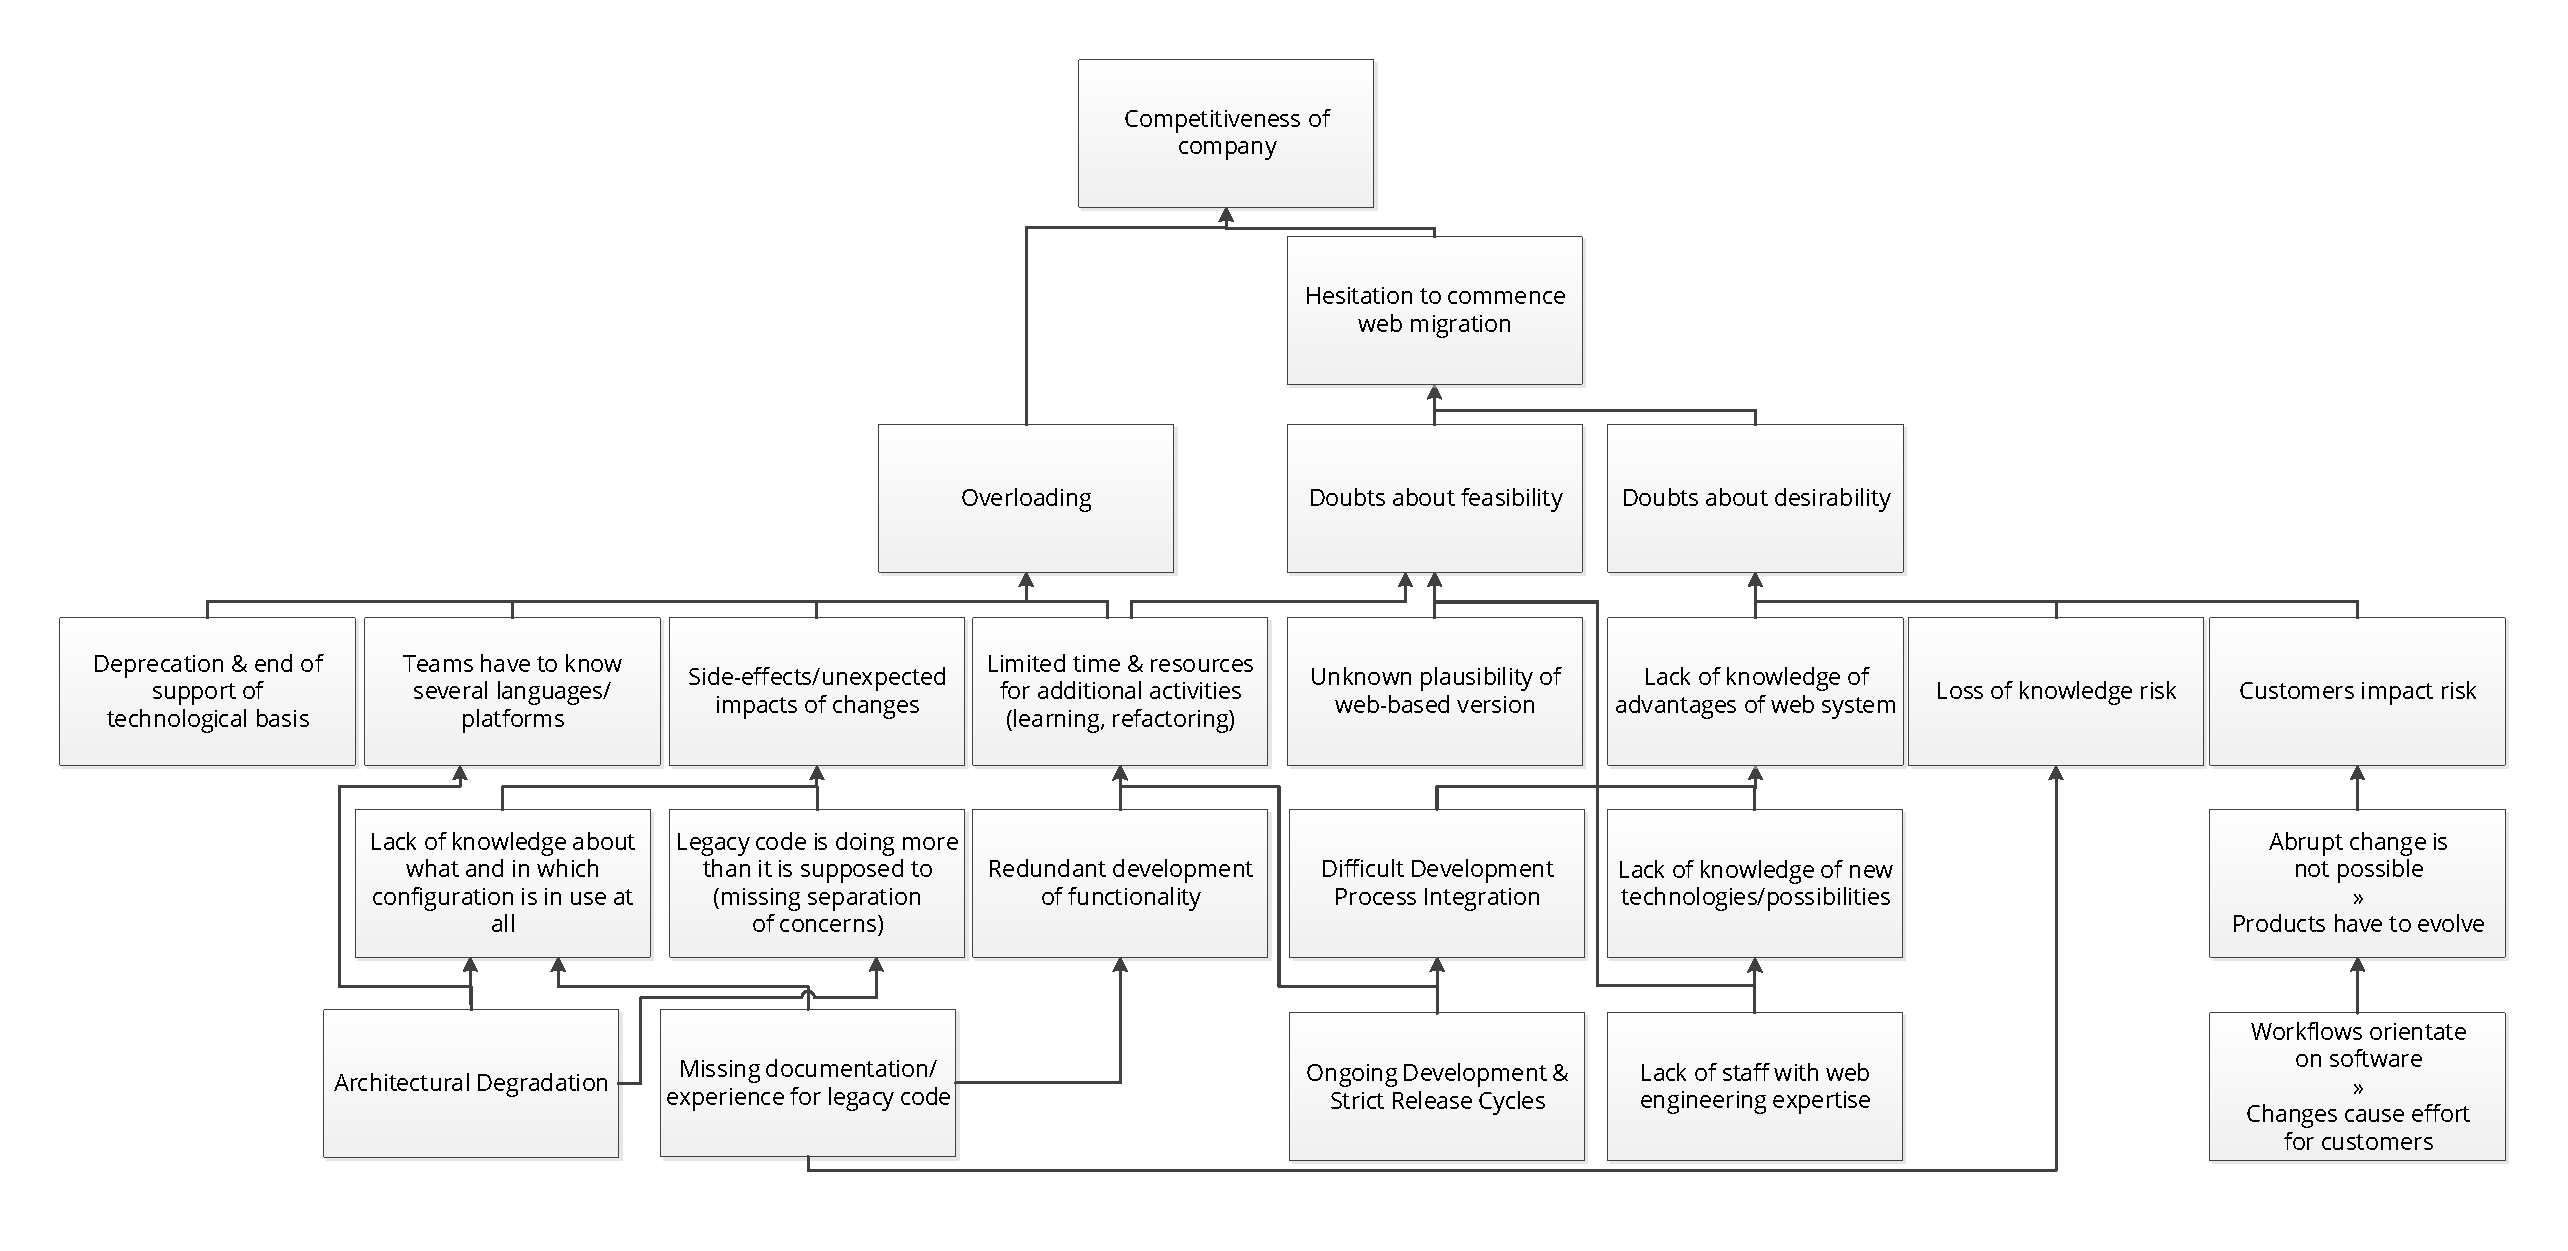
\includegraphics[width=0.99\textwidth]{../figures/20180115-DRF-Problem-Tree.pdf}
\caption{Hierarchical Representation of Problem Domain as LFA Problem Tree}\label{fig:problem-tree}
}
\end{sidewaysfigure}

\chapter{Solution Materials}
\begin{figure}[h!]
\hypertarget{fig:s2dcs-results}{%
\centering
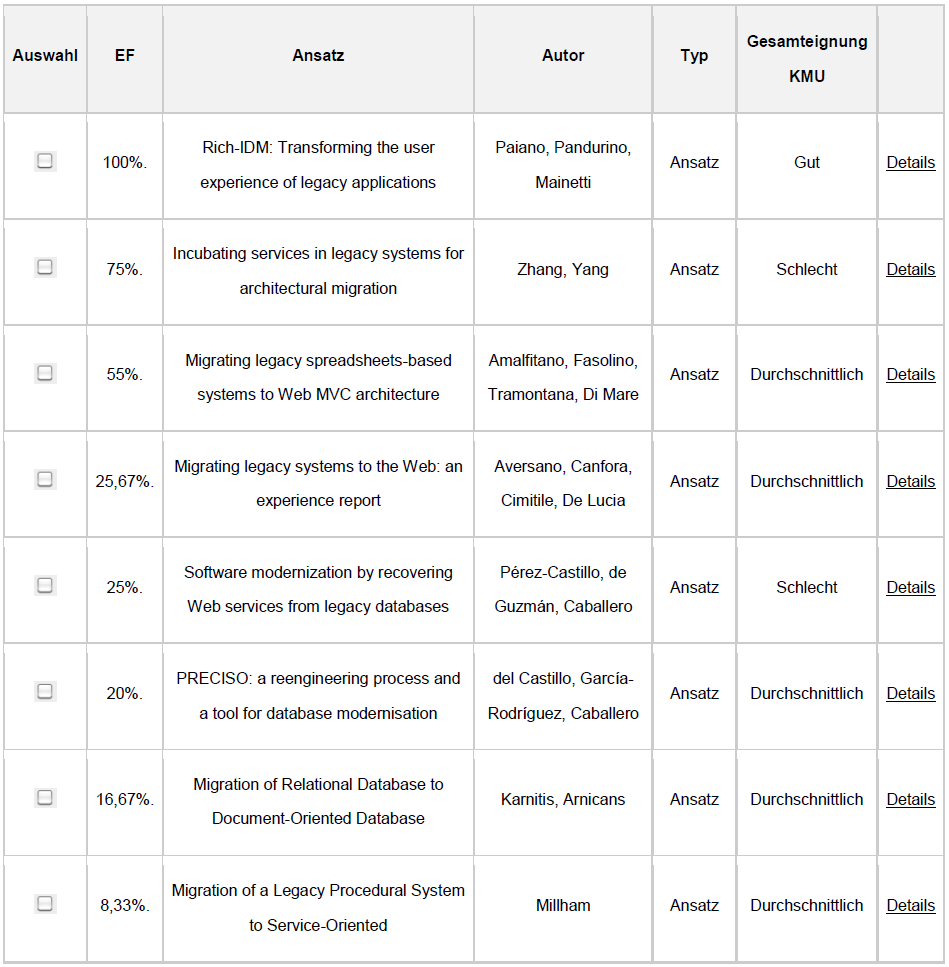
\includegraphics[width=0.78\textwidth]{../figures/screenshots/s2dcs-results.PNG}
\caption[S2DCS Results View]{S2DCS Results View, Showing Ranked List of Matching Approaches, EF Indicates Degree of Suitability to Migration Situation (German)}\label{fig:s2dcs-results}
}
\end{figure}

\begin{sidewaysfigure}[h!]
\hypertarget{fig:sckm-full}{%
\centering
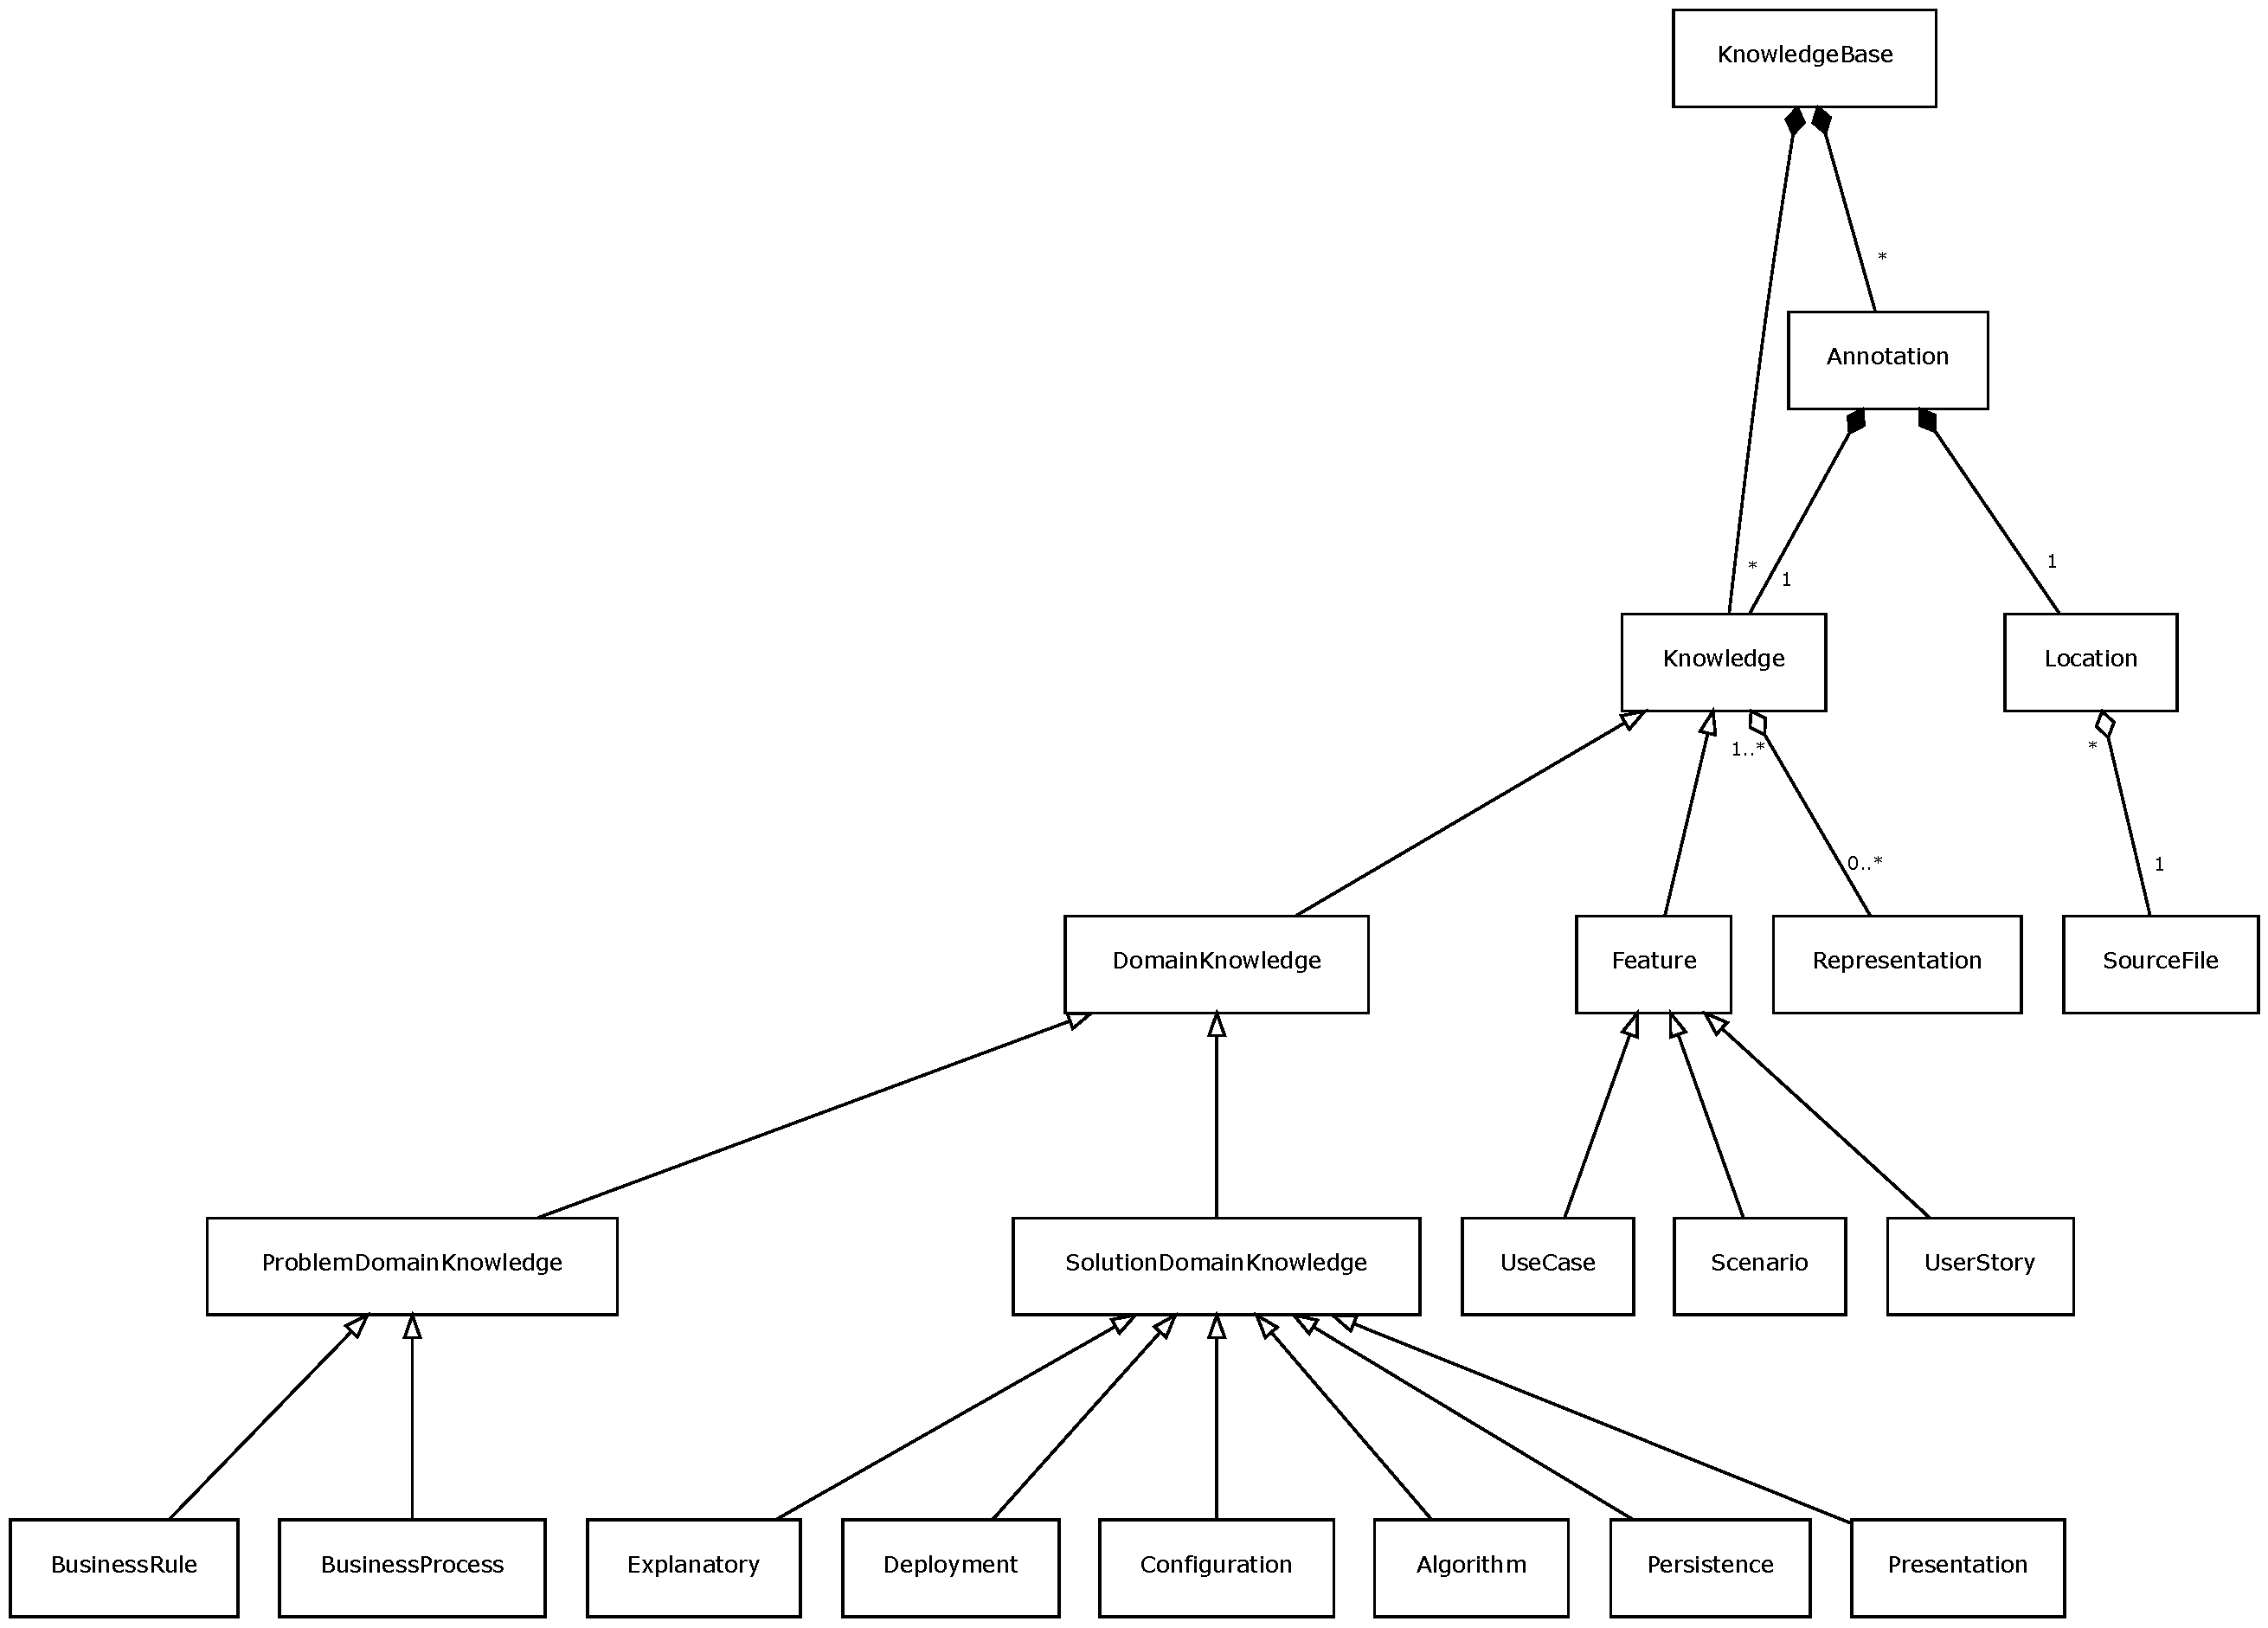
\includegraphics[width=0.82\textwidth]{../figures/sckm-full-uml.pdf}
\caption{SCKM Formalism}\label{fig:sckm-full}
}
\end{sidewaysfigure}

\chapter{AWSM:RE Materials}
\section{SCKM Ontology}\label{sec:sckm-ontology}
\vspace{15pt}
The following is an extract from the SCKM Ontology\footnote{available from the AWSM project page \url{https://vsr.informatik.tu-chemnitz.de/projects/2016/awsm/}} in Turtle notation. Since SWRL-Rules are very verbose in Turtle, they are shown separately in the following section.
\begin{lstlisting}[language=turtle, captionpos=t, caption=SCKM Ontology Extract]
@prefix : <https://vsr.informatik.tu-chemnitz.de/ontologies/source_knowledge#> .
@prefix oa: <http://www.w3.org/ns/oa#> .
@prefix kdm: <http://schema.omg.org/spec/KDM/1.2/kdm> .
@prefix owl: <http://www.w3.org/2002/07/owl#> .
@prefix rdf: <http://www.w3.org/1999/02/22-rdf-syntax-ns#> .
@prefix xml: <http://www.w3.org/XML/1998/namespace> .
@prefix xsd: <http://www.w3.org/2001/XMLSchema#> .
@prefix rdfs: <http://www.w3.org/2000/01/rdf-schema#> .
@prefix sckm: <https://vsr.informatik.tu-chemnitz.de/ontologies/source_knowledge#> .


@base <https://vsr.informatik.tu-chemnitz.de/ontologies/source_knowledge> .

<https://vsr.informatik.tu-chemnitz.de/ontologies/source_knowledge> rdf:type owl:Ontology.
                                                                
## Object Properties ##
oa:hasBody rdf:type owl:ObjectProperty ;
           rdfs:domain oa:Annotation ;
           rdfs:range sckm:DomainKnowledge ,
                      sckm:Feature .

oa:hasSelector rdf:type owl:ObjectProperty ;
               rdfs:domain oa:SpecificResource ;
               rdfs:range oa:TextPositionSelector ;
               rdfs:seeAlso <kdm:SourceRef> .

oa:hasTarget rdf:type owl:ObjectProperty ;
             rdfs:domain oa:Annotation ;
             rdfs:range oa:SpecificResource ;
             rdfs:seeAlso <kdm:SourceFile> .

sckm:influences rdf:type owl:ObjectProperty ;
                owl:inverseOf sckm:requires ;
                rdfs:domain sckm:DomainKnowledge ;
                rdfs:range sckm:Feature .

sckm:requires rdf:type owl:ObjectProperty ;
              rdfs:domain sckm:Feature ;
              rdfs:range sckm:DomainKnowledge .

sckm:within rdf:type owl:ObjectProperty ;
            rdfs:domain oa:Annotation ;
            rdfs:range sckm:Area .
            
## Data properties ##
oa:end rdf:type owl:DatatypeProperty ;
       rdfs:domain oa:TextPositionSelector ;
       rdfs:range xsd:integer .

oa:hasSource rdf:type owl:DatatypeProperty ;
             rdfs:domain oa:SpecificResource ;
             rdfs:range xsd:anyURI .

oa:start rdf:type owl:DatatypeProperty ;
         rdfs:domain oa:TextPositionSelector ;
         rdfs:range xsd:integer .

sckm:name rdf:type owl:DatatypeProperty ;
          rdfs:domain sckm:DomainKnowledge ,
                      sckm:Feature ;
          rdfs:range xsd:string .

## Classes ##
oa:Annotation rdf:type owl:Class ;
              rdfs:seeAlso <kdm:Annotation> .

oa:SpecificResource rdf:type owl:Class ;
                    owl:equivalentClass sckm:Area ;
                    rdfs:seeAlso <kdm:SourceFile> ,
                                 <kdm:SourceRef> .

oa:TextPositionSelector rdf:type owl:Class ;
                        rdfs:seeAlso <kdm:SourceRegion> .

sckm:Algorithm rdf:type owl:Class ;
               rdfs:subClassOf sckm:DomainKnowledge ;
               rdfs:seeAlso <kdm:BehaviorUnit> .

sckm:Area rdf:type owl:Class .

sckm:BusinessProccess rdf:type owl:Class ;
                      rdfs:subClassOf sckm:DomainKnowledge ;
                      rdfs:seeAlso <kdm:ConceptualFlow> .

sckm:Configuration rdf:type owl:Class ;
                   rdfs:subClassOf sckm:DomainKnowledge ;
                   rdfs:seeAlso <kdm:ConfigFile> .

sckm:Deployment rdf:type owl:Class ;
                rdfs:subClassOf sckm:DomainKnowledge .

sckm:DomainKnowledge rdf:type owl:Class .

sckm:Explanatory rdf:type owl:Class ;
                 rdfs:subClassOf sckm:DomainKnowledge ;
                 rdfs:seeAlso <kdm:CommentUnit> .

sckm:Feature rdf:type owl:Class .

sckm:Persistence rdf:type owl:Class ;
                 rdfs:subClassOf sckm:DomainKnowledge .

sckm:Presentation rdf:type owl:Class ;
                  rdfs:subClassOf sckm:DomainKnowledge .

sckm:Rule rdf:type owl:Class ;
          rdfs:subClassOf sckm:DomainKnowledge ;
          rdfs:seeAlso <kdm:RuleUnit> .
\end{lstlisting}
\vspace{-15pt}
\section{SCKM Ontology SWRL Rules}\label{sec:sckm-ontology-rules}
\vspace{15pt}

The following is an extract from the SCKM Ontology comprising its SWRL-Rules in SWRL Human Readable Syntax\footnote{cf.~\url{https://www.w3.org/Submission/SWRL/}}.
\begin{lstlisting}[language=turtle, captionpos=t, caption=SCKM Ontology SWRL Rules]
oa:Annotation(?AN) ^ sckm:Area(?AREA) ^ oa:hasTarget(?AN, ?SR) ^ oa:SpecificResource(?SR) ^ oa:hasSource(?SR, ?SOURCE) ^ oa:hasSource(?AREA, ?SOURCE) ^ oa:TextPositionSelector(?TAN) ^ oa:TextPositionSelector(?TAR) ^ oa:start(?TAN, ?san) ^ oa:start(?TAR, ?sar) ^ oa:end(?TAN, ?ean) ^ oa:end(?TAR, ?ear) ^ swrlb:lessThanOrEqual(?sar, ?san) ^ swrlb:greaterThanOrEqual(?ear, ?ean) -> sckm:within(?AN, ?AREA)

oa:start(?TR, ?sr) ^ oa:start(?TF, ?sf) ^ oa:hasSource(?SF, ?S) ^ oa:SpecificResource(?SR) ^ oa:TextPositionSelector(?TF) ^ oa:SpecificResource(?SF) ^ swrlb:lessThanOrEqual(?er, ?ef) ^ oa:Annotation(?AR) ^ swrlb:greaterThanOrEqual(?sr, ?sf) ^ oa:hasBody(?AF, ?F) ^ oa:hasBody(?AR, ?R) ^ oa:TextPositionSelector(?TR) ^ oa:hasSelector(?SF, ?TF) ^ oa:hasSelector(?SR, ?TR) ^ sckm:Feature(?F) ^ oa:end(?TR, ?er) ^ oa:end(?TF, ?ef) ^ oa:hasTarget(?AF, ?SF) ^ oa:hasTarget(?AR, ?SR) ^ oa:hasSource(?SR, ?S) ^ sckm:DomainKnowledge(?R) ^ oa:Annotation(?AF) -> sckm:requires(?F, ?R) ^ sckm:influences(?R, ?F)

oa:start(?TR, ?sr) ^ oa:start(?TF, ?sf) ^ oa:SpecificResource(?SR) ^ oa:TextPositionSelector(?TF) ^ oa:SpecificResource(?SF) ^ oa:Annotation(?AR) ^ oa:hasBody(?AF, ?F) ^ oa:hasBody(?AR, ?R) ^ oa:TextPositionSelector(?TR) ^ oa:hasSelector(?SF, ?TF) ^ oa:hasSelector(?SR, ?TR) ^ swrlb:lessThan(?sf, ?sr) ^ sckm:Feature(?F) ^ oa:end(?TR, ?er) ^ oa:end(?TF, ?ef) ^ oa:hasTarget(?AF, ?SF) ^ oa:hasTarget(?AR, ?SR) ^ swrlb:greaterThanOrEqual(?ef, ?sr) ^ swrlb:greaterThan(?er, ?ef) ^ sckm:DomainKnowledge(?R) ^ oa:Annotation(?AF) -> sckm:requires(?F, ?R) ^ sckm:influences(?R, ?F)

oa:start(?TR, ?sr) ^ oa:start(?TF, ?sf) ^ oa:SpecificResource(?SR) ^ oa:TextPositionSelector(?TF) ^ oa:SpecificResource(?SF) ^ swrlb:greaterThanOrEqual(?ef, ?er) ^ oa:Annotation(?AR) ^ oa:hasBody(?AF, ?F) ^ oa:hasBody(?AR, ?R) ^ oa:TextPositionSelector(?TR) ^ oa:hasSelector(?SF, ?TF) ^ oa:hasSelector(?SR, ?TR) ^ sckm:Feature(?F) ^ oa:end(?TR, ?er) ^ oa:end(?TF, ?ef) ^ oa:hasTarget(?AF, ?SF) ^ oa:hasTarget(?AR, ?SR) ^ swrlb:lessThanOrEqual(?sf, ?sr) ^ sckm:DomainKnowledge(?R) ^ oa:Annotation(?AF) -> sckm:requires(?F, ?R) ^ sckm:influences(?R, ?F)

oa:start(?TR, ?sr) ^ oa:start(?TF, ?sf) ^ swrlb:greaterThanOrEqual(?er, ?ef) ^ oa:SpecificResource(?SR) ^ oa:TextPositionSelector(?TF) ^ oa:SpecificResource(?SF) ^ oa:Annotation(?AR) ^ oa:hasBody(?AF, ?F) ^ oa:hasBody(?AR, ?R) ^ oa:TextPositionSelector(?TR) ^ oa:hasSelector(?SF, ?TF) ^ oa:hasSelector(?SR, ?TR) ^ swrlb:lessThanOrEqual(?sr, ?sf) ^ sckm:Feature(?F) ^ oa:end(?TR, ?er) ^ oa:end(?TF, ?ef) ^ oa:hasTarget(?AF, ?SF) ^ oa:hasTarget(?AR, ?SR) ^ sckm:DomainKnowledge(?R) ^ oa:Annotation(?AF) -> sckm:requires(?F, ?R) ^ sckm:influences(?R, ?F)

oa:start(?TR, ?sr) ^ oa:start(?TF, ?sf) ^ oa:hasSource(?SF, ?S) ^ oa:SpecificResource(?SR) ^ oa:TextPositionSelector(?TF) ^ oa:SpecificResource(?SF) ^ swrlb:greaterThanOrEqual(?ef, ?er) ^ oa:Annotation(?AR) ^ swrlb:lessThan(?sr, ?sf) ^ oa:hasBody(?AF, ?F) ^ oa:hasBody(?AR, ?R) ^ oa:TextPositionSelector(?TR) ^ oa:hasSelector(?SF, ?TF) ^ oa:hasSelector(?SR, ?TR) ^ swrlb:greaterThanOrEqual(?er, ?sf) ^ sckm:Feature(?F) ^ oa:end(?TR, ?er) ^ oa:end(?TF, ?ef) ^ oa:hasTarget(?AF, ?SF) ^ oa:hasTarget(?AR, ?SR) ^ oa:hasSource(?SR, ?S) ^ sckm:DomainKnowledge(?R) ^ oa:Annotation(?AF) -> sckm:requires(?F, ?R) ^ sckm:influences(?R, ?F)
\end{lstlisting}

\chapter{AWSM:RM Materials}

\begin{figure}[h]
	\centering
	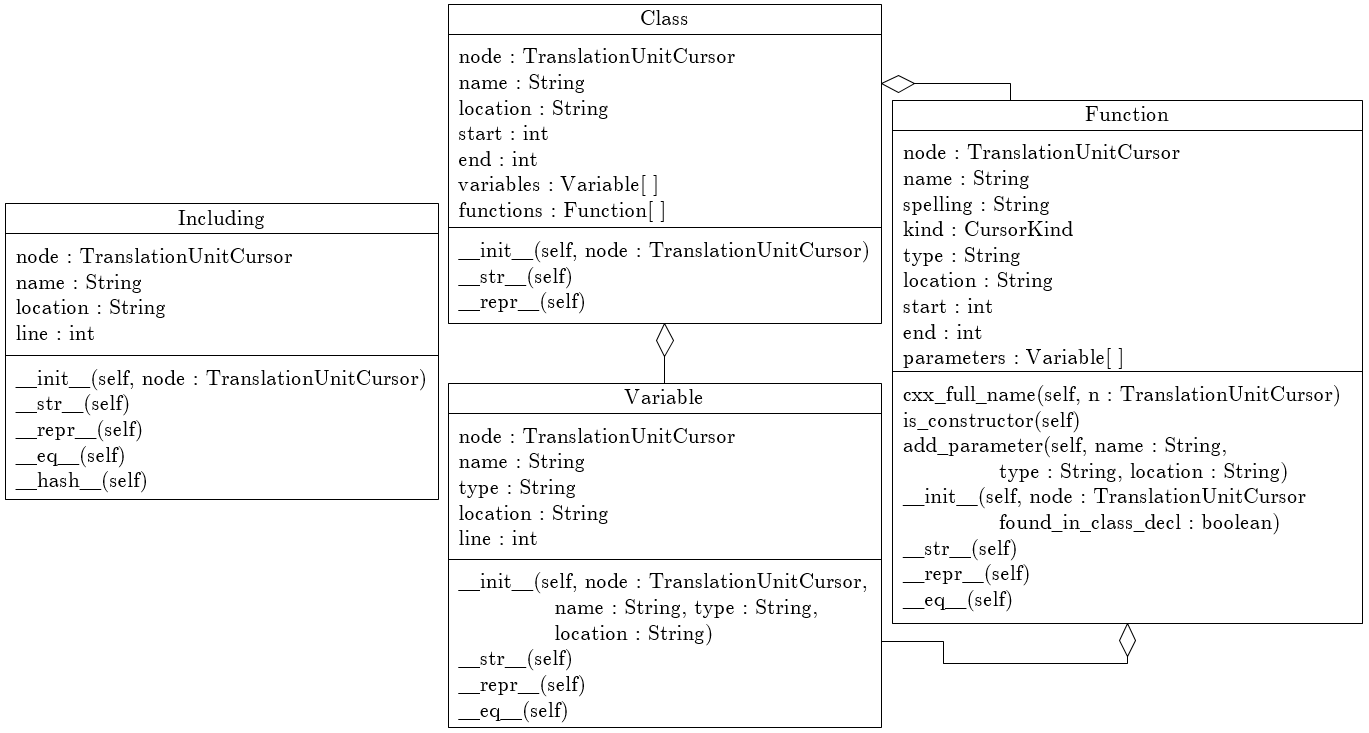
\includegraphics[width=0.99\textwidth]{rewamp/parserClasses}
	\caption{ReWaMP \cpp parser classes}
	\label{fig:rewamp-parser}
\end{figure}

\begin{table}[h]
\caption{ReWaMP Assumptions}
\label{tbl:rewamp-assump}
\centering
\def\arraystretch{1.35}
\setlength{\arrayrulewidth}{1.2pt}
\begin{tabularx}{\textwidth}{l X}
	Assumption & Description\\
	\hline
	Function Body & All functions start with one line as the header. Next, one line is possible starting with ':', but then the body starts. The first line of the body is only '\{' and the last only '\}'\\
	1 Return & All functions have only one return value. This infers that no changed parameter is needed after function's execution.\\
	UI IDs & The Web UI uses the old MFC ids. Not only the string versions, but also the integers in \emph{data-rwmpId}.\\
	File Size & All extracted files are relatively small and the number of extracted files is also manageable.\\
	Main Space & To find the name space of the view, the main file's name can be used. Searching all class names if including this name will match only at one class.\\
	Class Methods & All class functions are only declared in the class definition, but not defined.\\
	1 Name/Class & All class methods have a unique name inside of one class. Overriding functions by parameter lists is not present.\\
	No long long & No variables of the type long long or long double need to be exchanged with JS.\\
	Collections & Any collection as vector or map does not contain pointers of non-fundamental types and need be exchanged with JS.\\
	Pointers \& Vectors & If a vector is needs to be transferred from or to JS, there is only one pointer in the type. Types as 'vector<int*>*' thus are not needed at exchange. \\
%	Public Class Fields & All variables declared in a class are public accessible without getter or setter.\\
%	1 DoDataExchange & There is only one method DoDataExchange() in one view, and it is located in the main file. Further the only parameter is always called as in the MFC definition 'pDX'.\\
%	::GetFocus & In legacy code '::GetFocus()==' or '::GetFocus()!=' is only used in if-clauses.\\
%	.Format & '.Format' only appears at CString variables with '\%d'.\\
\end{tabularx}
\end{table}

\begin{sidewaysfigure}[h]
\hypertarget{fig:rwmpa-process}{%
\centering
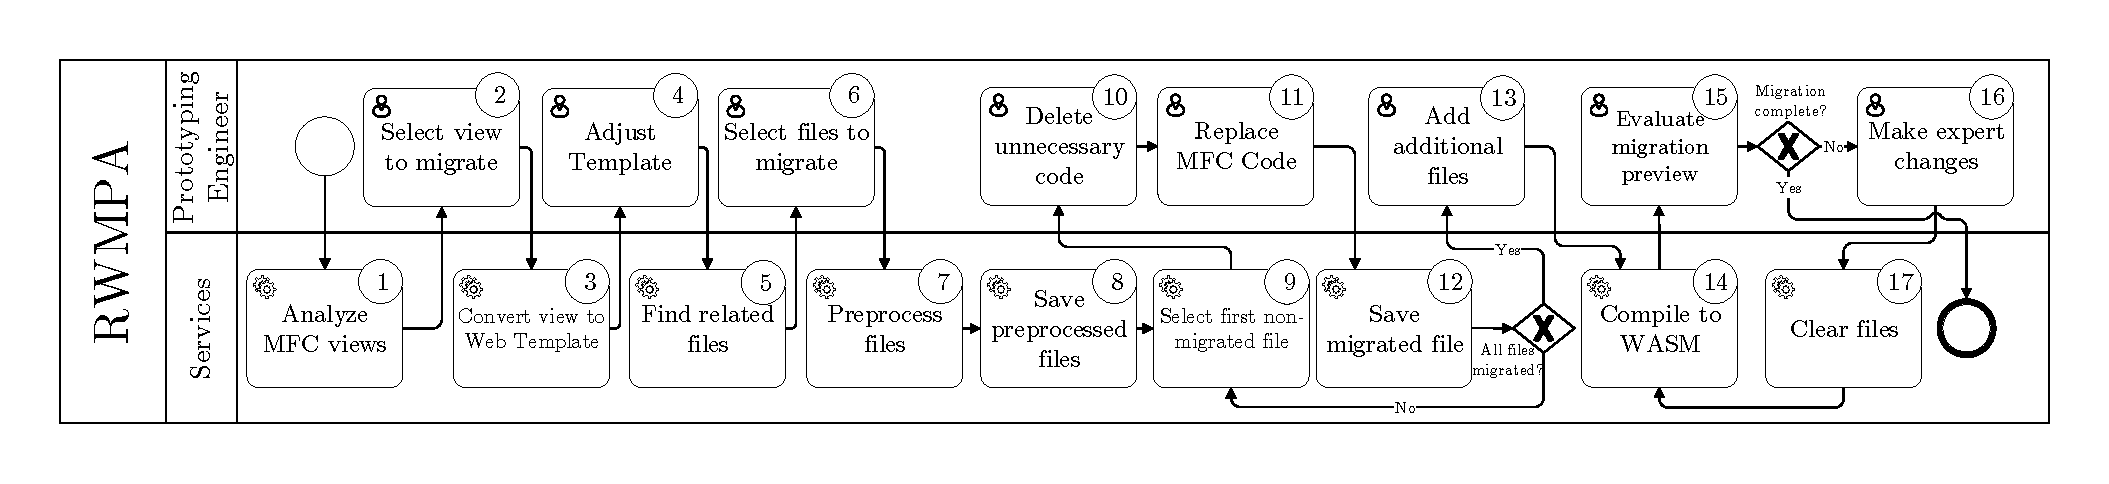
\includegraphics[width=0.99\textwidth]{../figures/rewamp/rwmpa-process.pdf}
\caption{RWMPA Process}\label{fig:rwmpa-process}
}
\end{sidewaysfigure}

\begin{figure}[h]
\hypertarget{fig:rwmpa-architecture}{%
\centering
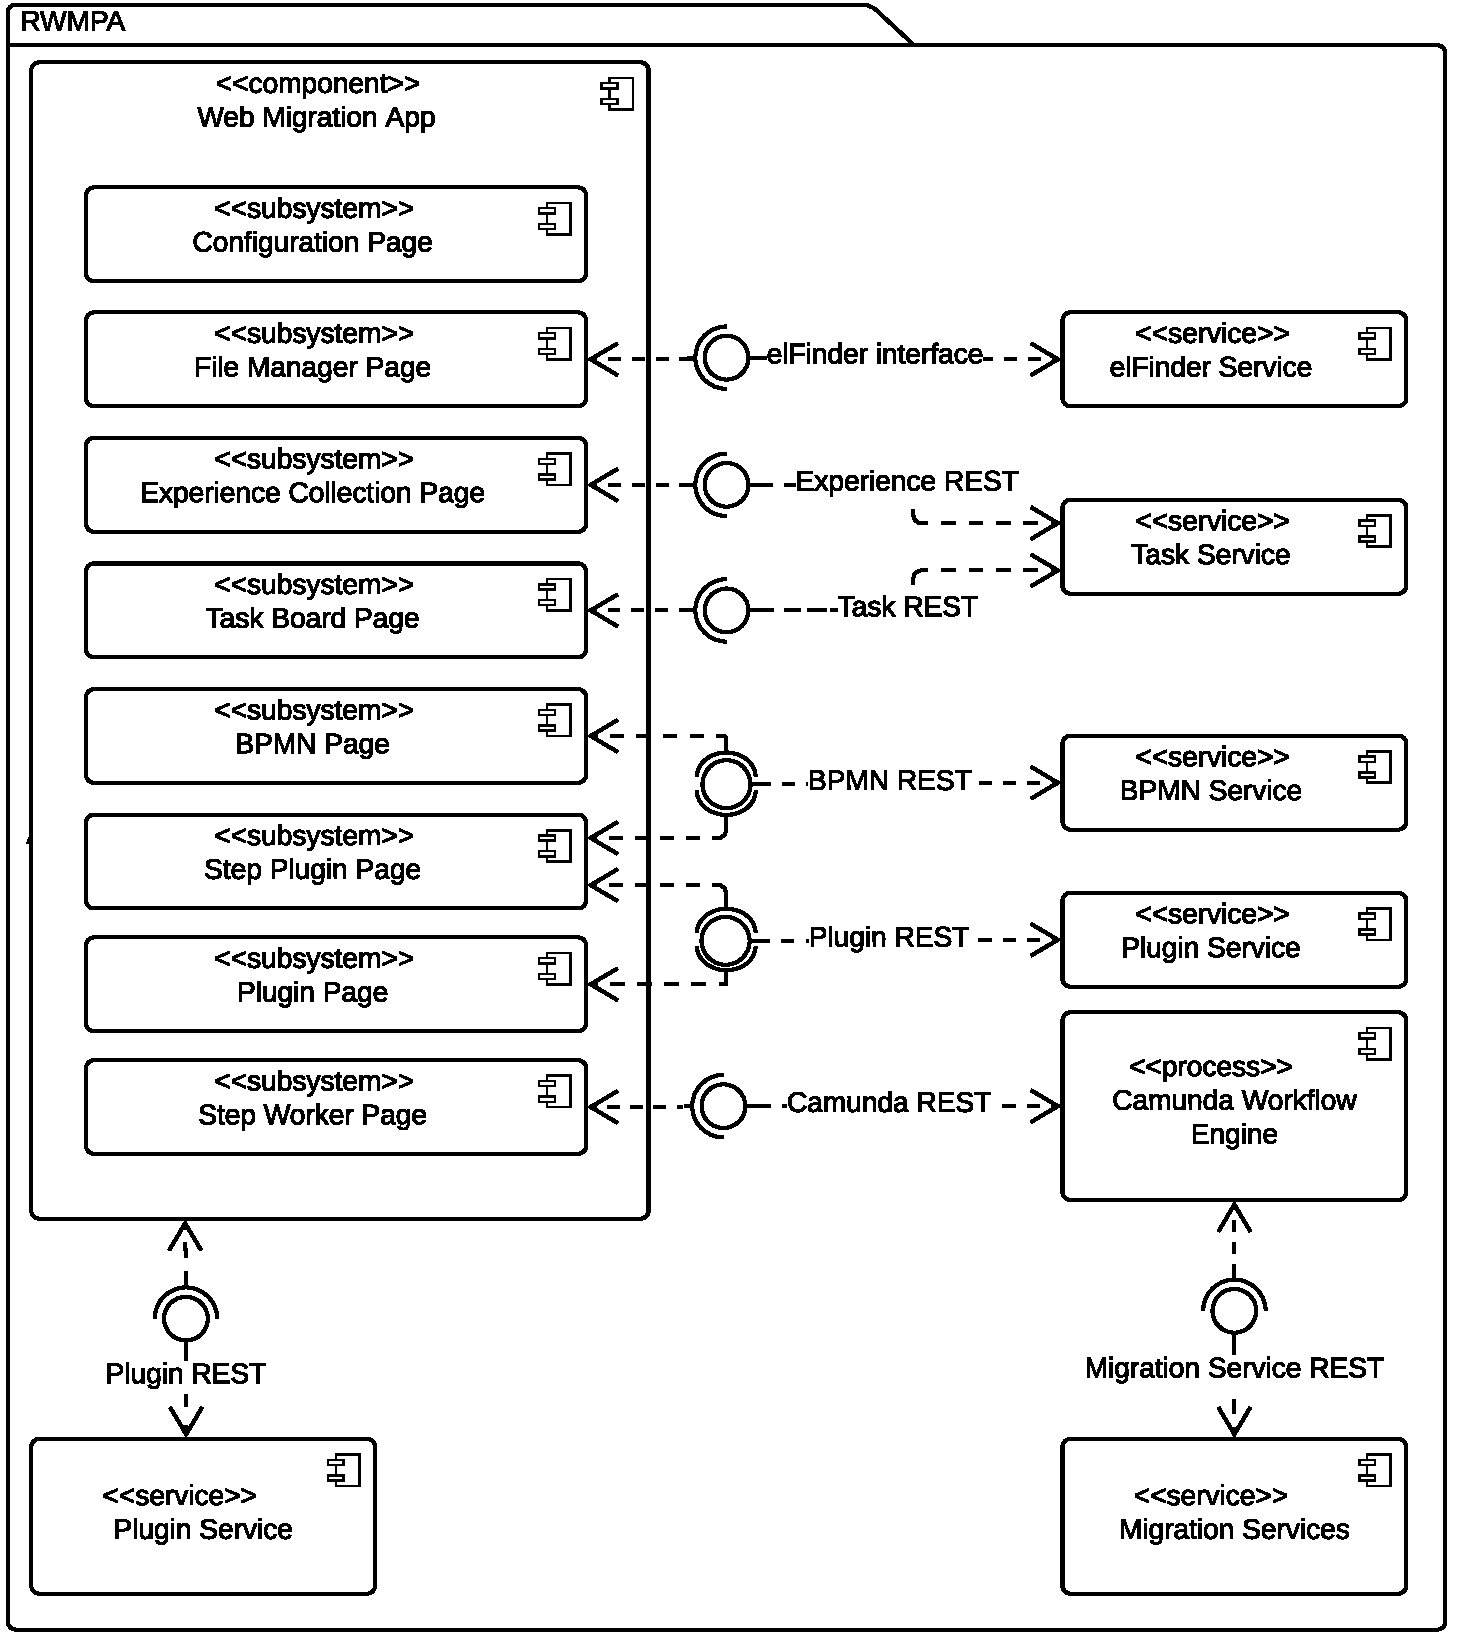
\includegraphics[width=0.9\textwidth]{../figures/rewamp/RWMPA-Architecture-NOFONTS.pdf}
\caption{RWMPA Architecture}\label{fig:rwmpa-architecture}
}
\end{figure}

\chapter{ReWaMP Evaluation Materials}
This appendix contains additional materials used in the ReWaMP evaluation experiments of this thesis.
\hypertarget{tbl:rewamp.guidelines}{}
\begin{longtable}[h]{@{}ll@{}}
\caption{ReWaMP Evaluation Guidelines}
\label{tbl:rewamp.guidelines}\tabularnewline
\toprule
\begin{minipage}[b]{0.17\columnwidth}\raggedright
Guideline\strut
\end{minipage} & \begin{minipage}[b]{0.77\columnwidth}\raggedright
Description\strut
\end{minipage}\tabularnewline
\midrule
\endfirsthead
\toprule
\begin{minipage}[b]{0.17\columnwidth}\raggedright
Guideline\strut
\end{minipage} & \begin{minipage}[b]{0.77\columnwidth}\raggedright
Description\strut
\end{minipage}\tabularnewline
\midrule
\endhead
\begin{minipage}[t]{0.17\columnwidth}\raggedright
Questions\strut
\end{minipage} & \begin{minipage}[t]{0.77\columnwidth}\raggedright
Answer all questions of the test subject, but stay as neutral and objective as possible.
The answer should not influence the test subject.\strut
\end{minipage}\tabularnewline
\begin{minipage}[t]{0.17\columnwidth}\raggedright
Syntax Errors\strut
\end{minipage} & \begin{minipage}[t]{0.77\columnwidth}\raggedright
Point out all apparent syntax errors a test subject made.
The note can be given to the test subject as soon as it continues in another line.\strut
\end{minipage}\tabularnewline
\begin{minipage}[t]{0.17\columnwidth}\raggedright
Misdirection\strut
\end{minipage} & \begin{minipage}[t]{0.77\columnwidth}\raggedright
Evince the test subject if it is apparently on the wrong way or performs useless actions.
So for example if the test subject reads in details about the data persistence implementation in action 1 instead of concentrating upon the task.\strut
\end{minipage}\tabularnewline
\begin{minipage}[t]{0.17\columnwidth}\raggedright
Expertise\strut
\end{minipage} & \begin{minipage}[t]{0.77\columnwidth}\raggedright
Help the test subject at missing programming experience or other program- ming issues.
Thereby it does not play a role if it is related to \cpp, MFC or Web development.
Only point out common structures, the support should not influence the test subject.\strut
\end{minipage}\tabularnewline
\bottomrule
\end{longtable}

\section{ReWaMP Questionaire\label{sec:rewamp-questionaire}}
\vspace{15pt}

The following questionaire was used in the experimental evaluation of ReWaMP in \cref{sec:rewamp.experiment}. Its structure and order of items represents the Google forms questionaire as seen by the test subjects. The specific questions used in the results analysis in \cref{sec:rewamp.experiment} are prefixed with Q1, Q2, Q3 etc. All statements are likert items on a 5 level scale of agreement from 1 - not at all to 5 - exactly. Items shown with indented subitems are corresponding to multiple-choice items, the last question of WASM-T group is a single-choice item.
\vspace{-15pt}

\subsection*{Self Assessment}
\begin{enumerate}
\item How many years of experience in programming do you have?
\item I have very much experience in web development.
\item I have very much experience in programming \cpp.
\item I have very much experience in using MFC for creating a GUI.
\end{enumerate}
\vspace{-15pt}

\subsection*{Functionality of Legacy System and ReWaMP Prototype}
\begin{enumerate}
\item In the legacy I am able to ...
\subitem browse the calendar
\subitem search all appointments of one patient
\subitem see all appointments at a specific date
\subitem find a new appointment by choosing a predefined variety
\subitem delete an existing appointment
\item In the resulting prototype I am able to ...
\subitem browse the calendar
\subitem search all appointments of one patient
\subitem see all appointments at a specific date
\subitem find a new appointment by choosing a predefined variety
\subitem delete an existing appointment
\end{enumerate}

\subsection*{Quality of Legacy System and ReWaMP Prototype}\vspace{-2pt}
\begin{enumerate}
\item In my opinion the legacy is performing just like I expected initially.
\item In my opinion the resulting prototype is performing just like I expected initially.
\item In my opinion the legacy is easy to use.
\item In my opinion the resulting prototype is easy to use.
\item In my opinion it is easy to learn how to use the legacy.
\item In my opinion it is easy to learn how to use the resulting prototype.
\end{enumerate}

\vspace{-20pt}
\subsection*{WASM-T}\vspace{-2pt}
\begin{enumerate}
\item\textbf{Q1} It was very easy to understand, what I have to do in the ReWaMP process.
\item WASM-T was very easy to use.
\item\textbf{Q2} I had to do a lot of manual work at the ReWaMP process.
\item\textbf{Q3} WASM-T carried off much work for me in the ReWaMP process.
\item\textbf{Q4} Without WASM-T the ReWaMP process would generate much more work for me.
\item\textbf{Q5} The ReWaMP process took me only a short amount of time.
\item\textbf{Q6} Without WASM-T the ReWaMP process would take me much longer.
\item WASM-T supported me very good at finding code fragments, which need an expert change.
\item WASM-T supported me at writing code fragments by offering ReWaMP flags.
\item WASM-T supported me very good at exporting functions to the server.
\item The most difficult task was for me...
\subitem Extract view related behavior files
\subitem Configure WASM-T
\subitem Make expert changes
\subitem Write expert file
\end{enumerate}

\vspace{-15pt}
\section{ReWaMP Evaluation Data}
\vspace{15pt}

\Cref{tbl:rewamp.empirical.full} contains the raw evaluation data of the empirical evaluation of ReWaMP, \cref{tbl:rewamp.times.full} the raw evaluation data from time measurements and \cref{tbl:rewamp.effort.full} from effort measurements.
%\pagebreak

%\begin{table}[h]
%\captionof{table}{Survey Overview\label{tab:overview}}
\begin{xltabular}[h]{\linewidth}{lllllll}
\caption[ReWaMP Full Empirical Evaluation Data]{ReWaMP Full Empirical Evaluation Data}\label{tbl:rewamp.empirical.full}\tabularnewline
\toprule
\textbf{Item} & \textbf{Sub 1} & \textbf{Sub 2} & \textbf{Sub 3} & \textbf{Sub 4} & \textbf{Sub 5} & \textbf{Sub 6} \tabularnewline
\midrule
\endfirsthead
\toprule
\textbf{Item} & \textbf{Sub 1} & \textbf{Sub 2} & \textbf{Sub 3} & \textbf{Sub 4} & \textbf{Sub 5} & \textbf{Sub 6} \tabularnewline
\midrule
\endhead
\small
S1 & 0 & 10 & 0 & 6 & 9 & 9\tabularnewline
S2 & 1 & 5 & 2 & 4 & 1 & 4\tabularnewline
S3 & 2 & 3 & 1 & 3 & 3 & 2\tabularnewline
S4 & 1 & 3 & 1 & 1 & 1 & 1\tabularnewline
F11 & Y & Y & Y & Y & Y & Y\tabularnewline
F12 & N & N & N & N & N & N\tabularnewline
F13 & Y & Y & Y & Y & Y & Y\tabularnewline
F14 & Y & Y & Y & Y & Y & Y\tabularnewline
F15 & N & N & N & N & N & N\tabularnewline
F21 & Y & Y & Y & Y & Y & Y\tabularnewline
F22 & N & N & N & N & N & N\tabularnewline
F23 & Y & Y & Y & Y & Y & Y\tabularnewline
F24 & Y & Y & Y & Y & Y & Y\tabularnewline
F25 & N & N & N & N & N & N\tabularnewline
Q1 & 4 & 2 & 3 & 5 & 3 & 2\tabularnewline
Q2 & 4 & 3 & 4 & 5 & 3 & 2\tabularnewline
Q3 & 4 & 2 & 2 & 4 & 4 & 2\tabularnewline
Q4 & 5 & 2 & 4 & 4 & 4 & 3\tabularnewline
Q5 & 5 & 3 & 2 & 5 & 5 & 4\tabularnewline
Q6 & 5 & 4 & 4 & 5 & 5 & 4\tabularnewline
W1 & 2 & 2 & 1 & 4 & 3 & 2\tabularnewline
W2 & 5 & 3 & 4 & 3 & 5 & 3\tabularnewline
W3 & 3 & 2 & 3 & 3 & 2 & 3\tabularnewline
W4 & 5 & 4 & 4 & 4 & 5 & 4\tabularnewline
W5 & 4 & 4 & 4 & 5 & 5 & 4\tabularnewline
W6 & 3 & 4 & 2 & 2 & 3 & 4\tabularnewline
W7 & 5 & 4 & 4 & 5 & 5 & 4\tabularnewline
W8 & 5 & 3 & 4 & 5 & 4 & 1\tabularnewline
W9 & 4 & 3 & 4 & 4 & 3 & 4\tabularnewline
W10 & 5 & 4 & 4 & 5 & 5 & 5\tabularnewline
W11 & 4 & 4 & 4 & 4 & 4 & 4\tabularnewline
\bottomrule
\caption*{Questionaire Responses, S1-S4 Self Assessment, F11-F25 Functionality, Q1-Q6 Quality, W1-W11 WASM-T, Abbreviations: Y - Yes, N - No}
\end{xltabular}
%\end{table}
\pagebreak

\begin{sidewaystable}[h!]
\begin{xltabular}{\linewidth}{llllllllllll}
\caption[ReWaMP Full Time Evaluation Data]{ReWaMP Full Time Evaluation Data}\label{tbl:rewamp.times.full}\tabularnewline
\toprule
\textbf{t1} & \textbf{t2} & \textbf{t31} & \textbf{t41} & \textbf{t51} & \textbf{t61} & \textbf{t71} & \textbf{t32} & \textbf{t42} & \textbf{t52} & \textbf{t62} & \textbf{t72} \tabularnewline
\midrule
\endfirsthead
\toprule
\textbf{t1} & \textbf{t2} & \textbf{t31} & \textbf{t41} & \textbf{t51} & \textbf{t61} & \textbf{t71} & \textbf{t32} & \textbf{t42} & \textbf{t52} & \textbf{t62} & \textbf{t72} \tabularnewline
\midrule
\endhead
\small
2319 & 230 & 17 & 2402 & 105 & 10 & 9 & 18 & 1924 & 531 & 21 & 11 \tabularnewline
673 & 106 & 18 & 1506 & 98 & 12 & 11 & 18 & 1536 & 456 & 21 & 12 \tabularnewline
1686 & 100 & 18 & 2425 & 159 & 12 & 18 & 18 & 2243 & 518 & 21 & 12 \tabularnewline
934 & 152 & 19 & 1788 & 70 & 13 & 14 & 18 & 1355 & 437 & 21 & 13 \tabularnewline
1560 & 166 & 18 & 2314 & 272 & 14 & 15 & 18 & 1314 & 415 & 21 & 11 \tabularnewline
1013 & 86 & 18 & 1949 & 132 & 14 & 13 & 19 & 1427 & 476 & 22 & 11 \tabularnewline
\bottomrule
\caption*{Measured times in seconds for tasks 1-7, tij indicates time for task i on view j}

\end{xltabular}

\begin{xltabular}{\linewidth}{lllllllllllllllll}
\caption[ReWaMP Full Effort Evaluation Data]{ReWaMP Full Effort Evaluation Data}\label{tbl:rewamp.effort.full}\tabularnewline
\toprule
\textbf{$\bm{e_{31}^{u}}$} & \textbf{$\bm{e_{31}^{d}}$} & \textbf{$\bm{e_{32}^{c}}$} & \textbf{$\bm{e_{32}^{u}}$} & \textbf{$\bm{e_{32}^{d}}$} & \textbf{$\bm{e_{41}^{c}}$} & \textbf{$\bm{e_{41}^{u}}$} & \textbf{$\bm{e_{41}^{d}}$} & \textbf{$\bm{e_{42}^{c}}$} & \textbf{$\bm{e_{42}^{u}}$} & \textbf{$\bm{e_{42}^{d}}$} & \textbf{$\bm{e_{51}^{c}}$} & \textbf{$\bm{e_{52}^{c}}$} &  \textbf{$\bm{e_{61}^{c}}$}  & \textbf{$\bm{e_{62}^{c}}$} &  \textbf{$\bm{e_{62}^{d}}$}  \tabularnewline
\midrule
\endfirsthead
\toprule
\textbf{$\bm{e_{31}^{u}}$} & \textbf{$\bm{e_{31}^{d}}$} & \textbf{$\bm{e_{32}^{c}}$} & \textbf{$\bm{e_{32}^{u}}$} & \textbf{$\bm{e_{32}^{d}}$} & \textbf{$\bm{e_{41}^{c}}$} & \textbf{$\bm{e_{41}^{u}}$} & \textbf{$\bm{e_{41}^{d}}$} & \textbf{$\bm{e_{42}^{c}}$} & \textbf{$\bm{e_{42}^{u}}$} & \textbf{$\bm{e_{42}^{d}}$} & \textbf{$\bm{e_{51}^{c}}$} & \textbf{$\bm{e_{52}^{c}}$} &  \textbf{$\bm{e_{61}^{c}}$}  & \textbf{$\bm{e_{62}^{c}}$} &  \textbf{$\bm{e_{62}^{d}}$}  \tabularnewline
\midrule
\endhead
\small
81 & 60 & 12 & 32 & 43 & 3 & 11 & 45 & 1 & 33 & 94 & 9 & 60 &  273 & 164 & 4  \tabularnewline
81 & 60 & 12 & 32 & 43 & 4 & 10 & 43 & 2 & 30 & 96 & 6 & 57 & 263 & 154 & 4  \tabularnewline
81 & 60 & 12 & 32 & 43 & 2 & 10 & 37 & 0 & 36 & 93 & 9 & 60 & 273 & 164 & 4  \tabularnewline
81 & 60 & 12 & 32 & 43 & 1 & 14 & 37 & 0 & 36 & 89 & 6 & 57 & 263 & 154 & 4  \tabularnewline
81 & 60 & 12 & 32 & 43 & 2 & 14 & 35 & 0 & 30 & 88 & 6 & 57 & 263 & 154 & 4  \tabularnewline
81 & 60 & 12 & 32 & 43 & 2 & 6 & 35 & 0 & 32 & 90 & 6 & 60 & 263 & 164 & 4  \tabularnewline
\bottomrule
\caption*{Measured efforts in SLOC for tasks 3-6, $e_{ij}^{a}$ indicates effort for action a on task i on view j, actions are c - create, u - update, d - delete, left out: $e_{51}^{u}$, $e_{51}^{d}$, $e_{52}^{u}$, $e_{52}^{d}$, $e_{61}^{d}$ (all values $0$), $e_{61}^{u}$ (all values $1$), $e_{31}^{c}$, $e_{62}^{u}$ (all values $9$)}
\addtocounter{table}{-1}

\end{xltabular}
\end{sidewaystable}

\chapter{RWMPA Evaluation Materials}
This appendix contains additional materials used in the RWMPA evaluation experiments of this thesis.

\hypertarget{tbl:rwmpa.guidelines}{}
\begin{longtable}[h]{@{}ll@{}}
\caption{RWMPA Evaluation Guidelines}\label{tbl:rwmpa.guidelines}\tabularnewline
\toprule
\begin{minipage}[b]{0.47\columnwidth}\raggedright
Situation\strut
\end{minipage} & \begin{minipage}[b]{0.47\columnwidth}\raggedright
Interaction\strut
\end{minipage}\tabularnewline
\midrule
\endfirsthead
\toprule
\begin{minipage}[b]{0.47\columnwidth}\raggedright
Situation\strut
\end{minipage} & \begin{minipage}[b]{0.47\columnwidth}\raggedright
Interaction\strut
\end{minipage}\tabularnewline
\midrule
\endhead
\begin{minipage}[t]{0.47\columnwidth}\raggedright
Test subject does not understand the task at hand\strut
\end{minipage} & \begin{minipage}[t]{0.47\columnwidth}\raggedright
The researcher points the test subject to the help section.
If the test subject still cannot understand the task, the researcher takes a note and explains the task.\strut
\end{minipage}\tabularnewline
\begin{minipage}[t]{0.47\columnwidth}\raggedright
Test subject writes a line with an apparent syntax error\strut
\end{minipage} & \begin{minipage}[t]{0.47\columnwidth}\raggedright
When the test subject continues to another line, the researcher points out the syntax errors to the test subject.\strut
\end{minipage}\tabularnewline
\begin{minipage}[t]{0.47\columnwidth}\raggedright
Test subjects wants to leave the RWMPA workflow before successful completion\strut
\end{minipage} & \begin{minipage}[t]{0.47\columnwidth}\raggedright
The researcher points out the problem to the test subject.
This situation can only occur in the final task of the RWMPA workflow: \emph{evaluate migration using a preview}.\strut
\end{minipage}\tabularnewline
\begin{minipage}[t]{0.47\columnwidth}\raggedright
Test subject gets stuck due to missing expertise.\strut
\end{minipage} & \begin{minipage}[t]{0.47\columnwidth}\raggedright
The researcher helps the test subject by providing knowledge on common structures, while not influence the decisions of the test subject.\strut
\end{minipage}\tabularnewline
\begin{minipage}[t]{0.47\columnwidth}\raggedright
Test subject runs the correction cycle at least twice because of ignoring the compiler errors\strut
\end{minipage} & \begin{minipage}[t]{0.47\columnwidth}\raggedright
The researcher points the test subject to the compiler errors and the possibility to reset the code to its original state.\strut
\end{minipage}\tabularnewline
\bottomrule
\end{longtable}

\vspace{-15pt}
\section{RWMPA Questionaire\label{sec:rwmpa-questionaire}}
\vspace{15pt}

The following questionaire was used in the experimental evaluation of RWMPA in \cref{sec:rwmpa.experiment}. 
Its structure and order of items represents the Google forms questionaire as seen by the test subjects. 
The specific questions used in the results analysis in \cref{sec:rwmpa.experiment} are prefixed with Q1, Q2, Q3 etc. All statements are likert items on a 5 level scale of agreement from 1 - not at all to 5 - exactly. 
Items shown with indented subitems are corresponding to single-choice items.
The original questionaire was in German language, the following text is a translation into English.

\subsection*{Self Assessment}
\begin{enumerate}
\item How many years of programming experience do you have?
\item I am very experienced in web development.
\item I am very experienced in development with \cpp.
\item I have already realized many projects using MFC.
\item My profession is ...
\end{enumerate}

\subsection*{Workflow}
\begin{enumerate}
\item \textbf{Q1} The workflow is easy to understand.
\item \textbf{Q2} I had to perform many manual edits.
\item \textbf{Q3} The workflow has reduced my work effort a lot
\item I required only little time for the workflow.
\item The workflow ran as I had expected. 
\item \textbf{Q7} The tools required manual configuration.
\item \textbf{Q4} The workflow guidance supported me in understanding the workflow.
\item I was always aware of where I am in the workflow.
\item The most difficult task was for me...
\subitem Select view to migrate
\subitem Adjust the template
\subitem Select files to migrate
\subitem Delete unnecessary source code from file
\subitem Replace MFC Code
\subitem Add additional files
\subitem Evaluate migration using a preview
\subitem Make expert changes
\subitem I do not remember
\item The number of tasks is...
\subitem Too high
\subitem Adequate
\subitem Too low
\end{enumerate}

\subsection*{Tasks}
\begin{enumerate}
\item \textbf{Q5} The task guidance supported me in understanding the tasks.
\item \textbf{Q6} I was constantly aware of what is to be done.
\item The GUI is very easy to use.
\item I had to refer to the help pages often.
\item I had to go back one task often.
\item I had to reset a task often.
\end{enumerate}

\section{RWMPA Evaluation Data}
\vspace{15pt}

\Cref{tbl:rwmpa.empirical.full} contains the raw evaluation data of the empirical evaluation of RWMPA, \cref{tbl:rwmpa.time.full} the raw data of the time measurements.

\begin{sidewaystable}[h!]
%\captionof{table}{Survey Overview\label{tab:overview}}
\begin{xltabular}{\linewidth}{lllllllllllll}
\caption[RWMPA Full Empirical Evaluation Data]{RWMPA Full Empirical Evaluation  Data}\label{tbl:rwmpa.empirical.full}\tabularnewline

\toprule
\textbf{S1} &\textbf{ S2} &\textbf{ S3} &\textbf{ S4} &\textbf{ S5} &\textbf{ W1} &\textbf{ W2} &\textbf{ W3} &\textbf{ W4} &\textbf{ W5} &\textbf{ W6} &\textbf{ W7} &\textbf{ W8} \tabularnewline
\midrule
\endfirsthead
\toprule
\textbf{S1} &\textbf{ S2} &\textbf{ S3} &\textbf{ S4} &\textbf{ S5} &\textbf{ W1} &\textbf{ W2} &\textbf{ W3} &\textbf{ W4} &\textbf{ W5} &\textbf{ W6} &\textbf{ W7} &\textbf{ W8} \tabularnewline
\midrule
\endhead
\small
7 & 2 & 2 & 1 & Student & 5 & 2 & 4 & 5 & 4 & 1 & 5 & 4 \tabularnewline
10 & 2 & 3 & 1 & Student & 4 & 3 & 4 & 3 & 4 & 2 & 5 & 5 \tabularnewline
9 & 2 & 3 & 2 & Researcher & 3 & 3 & 4 & 4 & 4 & 1 & 4 & 3 \tabularnewline
15 & 3 & 2 & 1 & SW Architect & 4 & 3 & 3 & 4 & 4 & 3 & 2 & 5 \tabularnewline
15 & 5 & 2 & 1 & SW Engineer & 3 & 4 & 3 & 3 & 3 & 1 & 4 & 3 \tabularnewline
9 & 2 & 2 & 1 & Student & 5 & 2 & 5 & 4 & 5 & 1 & 5 & 5 \tabularnewline
7 & 3 & 1 & 1 & Studen & 4 & 3 & 5 & 4 & 4 & 2 & 4 & 4 \tabularnewline

\bottomrule
\caption*{Questionaire responses, S1-S5 Self Assessment, W1-W8 Workflow}

\end{xltabular}

\begin{xltabular}{\linewidth}{lllllllllllll}
\caption[RWMPA Full Empirical Evaluation Data (cont.)]{RWMPA Full Empirical Evaluation Data (cont.)}\label{tbl:rwmpa.empirical.full.2}\tabularnewline

\toprule
\textbf{ W9} &\textbf{ W10} &\textbf{ T1} &\textbf{ T2} &\textbf{ T3} &\textbf{ T4} &\textbf{ T5} & \textbf{T6}\tabularnewline
\midrule
\endfirsthead
\toprule
\textbf{ W9} &\textbf{ W10} &\textbf{ T1} &\textbf{ T2} &\textbf{ T3} &\textbf{ T4} &\textbf{ T5} & \textbf{T6}\tabularnewline
\midrule
\endhead
\small
16 & Adq. & 5 & 4 & 5 & 1 & 2 & 1 \tabularnewline
11 & Adq & 5 & 4 & 4 & 1 & 2 & 2 \tabularnewline
11 & Adq & 3 & 3 & 3 & 4 & 3 & 1 \tabularnewline
16 & TH & 3 & 3 & 5 & 1 & 2 & 1 \tabularnewline
16 & Adq & 4 & 4 & 5 & 2 & 2 & 2 \tabularnewline
11 & Adq & 5 & 4 & 5 & 2 & 1 & 1 \tabularnewline
16 & Adq & 4 & 4 & 5 & 3 & 2 & 2 \tabularnewline

\bottomrule
\caption*{Questionaire responses, W9-W10 Workflow, T1-T6 Tasks, Abbreviations: SW - Software, ADQ - Adequate, TH - Too high}

\end{xltabular}
\end{sidewaystable}

\begin{sidewaystable}[h!]
\begin{xltabular}{\linewidth}{lllllllllllllll}
\caption[RWMPA Full Time Evaluation Data]{RWMPA Full Time Evaluation Data}\label{tbl:rwmpa.time.full}\tabularnewline
\toprule
\textbf{t2.1} & \textbf{t4.1} & \textbf{t6.1} & \textbf{t10.1} & \textbf{t11.1} & \textbf{t13.1} & \textbf{t15.1} & \textbf{t16.1} & \textbf{t2.2} & \textbf{t4.2} \tabularnewline
\midrule
\endfirsthead
\toprule
\textbf{t2.1} & \textbf{t4.1} & \textbf{t6.1} & \textbf{t10.1} & \textbf{t11.1} & \textbf{t13.1} & \textbf{t15.1} & \textbf{t16.1} & \textbf{t2.2} & \textbf{t4.2} \tabularnewline
\midrule
\endhead
\small
255 & 131 & 90 & 273 & 1298 & 150 & 284 & 121 & 11 & 37 \tabularnewline
274 & 20 & 110 & 125 & 1525 & 41 & 155 & 97 & 3 & 2 \tabularnewline
275 & 58 & 36 & 187 & 1153 & 50 & 129 & 118 & 4 & 58 \tabularnewline
334 & 94 & 86 & 123 & 1093 & 66 & 258 & 105 & N/A & N/A \tabularnewline
230 & 270 & 183 & 333 & 1150 & 97 & 435 & 141 & N/A & N/A \tabularnewline
283 & 135 & 127 & 280 & 1703 & 241 & 284 & 249 & 13 & 22 \tabularnewline
227 & 123 & 114 & 179 & 1510 & 283 & 210 & 352 & 3 & 21 \tabularnewline
\bottomrule
\caption*{Times for manual tasks in seconds, ti.j - time for task i on view j, view 1: $u_{cal}$, view 2: $u_{new}$, N/A - not available}
\end{xltabular}

\begin{xltabular}{\linewidth}{llllll}
\caption[RWMPA Full Time Evaluation Data (cont.)]{RWMPA Full Time Evaluation Data (cont.)}\label{tbl:rwmpa.time.full.2}\tabularnewline
\toprule
\textbf{t6.2} & \textbf{t10.2} & \textbf{t11.2} & \textbf{t13.2} & \textbf{t15.2} & \textbf{t16.2} \tabularnewline
\midrule
\endfirsthead
\toprule
\textbf{t6.2} & \textbf{t10.2} & \textbf{t11.2} & \textbf{t13.2} & \textbf{t15.2} & \textbf{t16.2} \tabularnewline
\midrule
\endhead
\small
17 & 34 & 775 & 22 & 190 & 704 \tabularnewline
56 & 56 & 503 & 25 & 212 & 745 \tabularnewline
63 & 29 & 378 & 16 & 110 & 803 \tabularnewline
N/A & N/A & N/A & N/A & N/A & N/A \tabularnewline
N/A & N/A & N/A & N/A & N/A & N/A \tabularnewline
13 & 12 & 697 & 10 & 280 & 959 \tabularnewline
82 & 8 & 651 & 17 & 207 & 1045 \tabularnewline
\bottomrule
\caption*{Times for manual tasks in seconds, ti.j - time for task i on view j, view 1: $u_{cal}$, view 2: $u_{new}$, N/A - not available}
\addtocounter{table}{-1}
\end{xltabular}
\end{sidewaystable}

\chapter{UI Transformer Evaluation Materials}
This appendix contains additional materials used in the UI Transformer evaluation experiments of this thesis.
\vspace{-15pt}
\section{UI Transformer Questionaire\label{sec:uitransformer-questionaire}}
\vspace{15pt}

The following questionaire was used in the experimental evaluation of RWMPA in \cref{sec:uitransformer.experiment}. 
Its structure and order of items represents the Google forms questionaire as seen by the test subjects, the numbering of items is equivalent to the numbers used in the results analysis in \cref{sec:rwmpa.experiment}. 
All statements are likert items on a 5 level scale of agreement from 1 - strongly disagree to 5 - strongly agree. 
Items shown with indented subitems are corresponding to single-choice items.
The original questionaire was in German language, the following text is a translation into English.

\subsection*{Task Description}

Task: Compare the graphical user interface A with the graphical user interface B.
It is not necessary to look for each small difference; only those which stand out are sufficient.

After the comparison, assess the following statements.
There are no right or wrong answers.

\subsection*{Questions}
\begin{enumerate}[start=1,label={\bfseries Q\arabic*}]
\item The elements in A and B are of equal size.
\item The elements in A are at least as large as the elements in B.
\item Left aligned elements in A are also left aligned in B.
\item Right aligned elements in A are also right aligned in B.
\item The elements in A and B were assigned the same labels.
\item The elements in A and B occur in the same order.
\item A and B are identical.
\end{enumerate}

\vspace{-15pt}
\section{UI Transformer Evaluation Data}
\vspace{15pt}
\Cref{tbl:uitransformer.fullperformance} comprises the raw evaluation data of the performance evaluation and \cref{tbl:uitransformer.fullempirical} of the empirical evaluation of UI Transformer.

\begin{landscape}
%\captionof{table}{Survey Overview\label{tab:overview}}
\begin{xltabular}{\linewidth}{llllllllllllll}
\caption[UITransformer Performance Evaluation Data]{UITransformer Performance Evaluation Data}\label{tbl:uitransformer.fullperformance}\tabularnewline
\toprule
$\bm{i}$ & $\bm{\#c}$ & $\bm{d}$ & $\bm{t_1}$ & $\bm{t_2}$ & $\bm{t_3}$ & $\bm{t_4}$ & $\bm{t_5}$ & $\bm{t_6}$\tabularnewline
\midrule
\endfirsthead
\toprule
$\bm{i}$ & $\bm{\#c}$ & $\bm{d}$ & $\bm{t_1}$ & $\bm{t_2}$ & $\bm{t_3}$ & $\bm{t_4}$ & $\bm{t_5}$ & $\bm{t_6}$\tabularnewline
\midrule
\endhead
\small
1 & 23 & 0 & 52991 & 68519 & 104155 & 109407 & 141808 & 39902\tabularnewline
2 & 3 & 0 & 16279 & 15478 & 28198 & 36613 & 45745 & 12307\tabularnewline
3 & 20 & 1 & 54291 & 65815 & 100514 & 103873 & 124564 & 39784\tabularnewline
4 & 10 & 1 & 34085 & 33375 & 51327 & 56723 & 83637 & 25141\tabularnewline
5 & 24 & 1 & 70494 & 93683 & 136509 & 138137 & 225771 & 49583\tabularnewline
6 & 16 & 0 & 43013 & 46811 & 72981 & 89444 & 132452 & 31102\tabularnewline
7 & 17 & 0 & 45297 & 52942 & 74969 & 77915 & 108202 & 32471\tabularnewline
8 & 11 & 0 & 34845 & 36229 & 57637 & 63544 & 89369 & 24338\tabularnewline
9 & 9 & 1 & 30242 & 36700 & 60202 & 66611 & 108856 & 23185\tabularnewline
10 & 44 & 0 & 90796 & 120752 & 172615 & 164410 & 280721 & 72676\tabularnewline
11 & 21 & 0 & 54963 & 68549 & 90554 & 104358 & 171898 & 38218\tabularnewline
12 & 8 & 0 & 27163 & 26802 & 41923 & 50756 & 73983 & 19923\tabularnewline
13 & 13 & 0 & 37060 & 39273 & 61597 & 64808 & 116680 & 26815\tabularnewline
14 & 34 & 1 & 89702 & 126699 & 174827 & 182356 & 293741 & 66420\tabularnewline
15 & 18 & 0 & 47694 & 53825 & 77801 & 83897 & 133893 & 34807\tabularnewline
16 & 18 & 0 & 47282 & 55174 & 76268 & 86177 & 127002 & 34545\tabularnewline
17 & 17 & 0 & 45746 & 53665 & 81786 & 83927 & 134995 & 33211\tabularnewline
18 & 26 & 0 & 66019 & 80763 & 117248 & 121745 & 179148 & 46401\tabularnewline
19 & 15 & 0 & 40564 & 46082 & 63594 & 70852 & 110924 & 30169\tabularnewline
20 & 45 & 0 & 104418 & 148559 & 204541 & 211551 & 355712 & 74151\tabularnewline
21 & 25 & 0 & 65858 & 76207 & 111911 & 112844 & 186624 & 46118\tabularnewline
22 & 17 & 1 & 54653 & 66542 & 97983 & 105352 & 148268 & 41912\tabularnewline
23 & 9 & 0 & 28687 & 28396 & 44376 & 48115 & 71211 & 20889\tabularnewline
24 & 15 & 0 & 41959 & 46156 & 71397 & 71739 & 116134 & 30523\tabularnewline
25 & 24 & 0 & 63211 & 72244 & 122268 & 111309 & 162568 & 43332\tabularnewline
26 & 12 & 0 & 35509 & 39687 & 58831 & 62721 & 112413 & 25747\tabularnewline
27 & 7 & 0 & 24856 & 23416 & 41805 & 45161 & 60975 & 18517\tabularnewline
28 & 23 & 0 & 58854 & 67693 & 114172 & 107139 & 176296 & 42199 \tabularnewline
29 & 2 & 0 & 13826 & 11275 & 19827 & 26228 & 32520 & 11046\tabularnewline
30 & 18 & 0 & 45411 & 53378 & 82518 & 83866 & 129468 & 34244\tabularnewline
31 & 4 & 0 & 18772 & 17917 & 30647 & 37269 & 49093 & 14107\tabularnewline
32 & 13 & 0 & 36239 & 39781 & 61251 & 70590 & 99885 & 27315\tabularnewline
33 & 15 & 0 & 39338 & 44354 & 61204 & 68855 & 118620 & 30102\tabularnewline
34 & 5 & 0 & 20911 & 18955 & 33715 & 40593 & 60701 & 15633\tabularnewline
35 & 33 & 0 & 78749 & 98299 & 127206 & 150440 & 200350 & 57718\tabularnewline
36 & 33 & 0 & 79973 & 110052 & 141222 & 150619 & 250577 & 57913\tabularnewline
37 & 44 & 0 & 101350 & 134914 & 205079 & 182565 & 272043 & 73661\tabularnewline
38 & 26 & 1 & 64573 & 90133 & 125346 & 127640 & 166848 & 47770\tabularnewline
39 & 130 & 0 & 343834 & 454761 & 532608 & 519752 & 1040988 & 312285\tabularnewline
40 & 44 & 0 & 99871 & 139913 & 182475 & 191001 & 331185 & 72570\tabularnewline
41 & 14 & 0 & 39149 & 42180 & 65693 & 74368 & 114644 & 28589\tabularnewline
42 & 59 & 0 & 132403 & 196759 & 265300 & 274095 & 484474 & 101199\tabularnewline
43 & 17 & 0 & 45233 & 52882 & 80782 & 87955 & 134987 & 33102\tabularnewline
44 & 9 & 1 & 32129 & 35214 & 54621 & 62866 & 85028 & 23750\tabularnewline
45 & 19 & 1 & 60210 & 84253 & 125042 & 123651 & 200841 & 44536\tabularnewline
46 & 30 & 1 & 85789 & 122708 & 179650 & 178399 & 302888 & 62849\tabularnewline
47 & 18 & 2 & 56963 & 75345 & 106238 & 114095 & 191564 & 43156\tabularnewline
48 & 24 & 1 & 70606 & 101166 & 135809 & 145739 & 158754 & 54125\tabularnewline
49 & 19 & 2 & 63455 & 86677 & 136162 & 140005 & 241658 & 47643\tabularnewline
50 & 22 & 1 & 66127 & 79544 & 109946 & 111316 & 181482 & 49496\tabularnewline
\bottomrule
\caption*{$i$ - index of layout $l_i$, $\#c$ - number of controls, $d$ - maximum nested depth, $t_j$ - transformation time for combination $j$ in ms}

\end{xltabular}

\begin{xltabular}{\linewidth}{llllllllllllll}
\caption[UITransformer Performance Evaluation Data (cont.)]{UITransformer Performance Evaluation Data (cont.)}\label{tbl:uitransformer.fullperformance.2}\tabularnewline
\toprule
$\bm{i}$ & $\bm{t_{6c}}$ & $\bm{t_7}$ & $\bm{t_8}$ & $\bm{t_9}$ & $\bm{t_{10}}$\tabularnewline
\midrule
\endfirsthead
\toprule
$\bm{i}$ & $\bm{t_{6c}}$ & $\bm{t_7}$ & $\bm{t_8}$ & $\bm{t_9}$ & $\bm{t_{10}}$\tabularnewline
\midrule
\endhead
\small
1 & 935 & 124686 & 112758 & 125425 & 203952 \tabularnewline
2 & 82 & 37245 & 27874 & 36292 & 57693 \tabularnewline
3 & 1217 & 123189 & 113321 & 115981 & 172955 \tabularnewline
4 & 506 & 68264 & 54769 & 65621 & 100792 \tabularnewline
5 & 2040 & 171170 & 128068 & 158620 & 208725 \tabularnewline
6 & 597 & 97152 & 74642 & 88178 & 142336 \tabularnewline
7 & 620 & 88533 & 74403 & 83224 & 136986 \tabularnewline
8 & 361 & 73976 & 59159 & 55261 & 111850 \tabularnewline
9 & 436 & 77622 & 49378 & 75228 & 119490 \tabularnewline
10 & 2647 & 206337 & 169370 & 184588 & 321439 \tabularnewline
11 & 850 & 114961 & 102480 & 101643 & 178151 \tabularnewline
12 & 231 & 57956 & 41112 & 55115 & 95696 \tabularnewline
13 & 419 & 84170 & 65159 & 73083 & 128390 \tabularnewline
14 & 3239 & 238330 & 178803 & 216341 & 302040 \tabularnewline
15 & 689 & 100739 & 77360 & 80813 & 165599 \tabularnewline
16 & 674 & 101801 & 78763 & 89394 & 142913 \tabularnewline
17 & 623 & 103131 & 74524 & 93218 & 156199 \tabularnewline
18 & 1136 & 146010 & 116134 & 122263 & 224872 \tabularnewline
19 & 524 & 83245 & 64305 & 76411 & 128667 \tabularnewline
20 & 2645 & 269510 & 194894 & 227905 & 374662 \tabularnewline
21 & 1088 & 138377 & 96956 & 115449 & 205943 \tabularnewline
22 & 1691 & 114799 & 92023 & 90833 & 169773 \tabularnewline
23 & 273 & 55916 & 42943 & 50188 & 87356 \tabularnewline
24 & 532 & 89160 & 63933 & 73353 & 144680 \tabularnewline
25 & 1051 & 137168 & 103691 & 118977 & 214945 \tabularnewline
26 & 391 & 72834 & 57766 & 75042 & 128375 \tabularnewline
27 & 204 & 53822 & 39313 & 46733 & 79825 \tabularnewline
28 & 984 & 117695 & 94551 & 107629 & 229665 \tabularnewline
29 & 62 & 26766 & 20692 & 24792 & 42196 \tabularnewline
30 & 661 & 105192 & 80027 & 95523 & 182402 \tabularnewline
31 & 107 & 38928 & 30270 & 37001 & 63937 \tabularnewline
32 & 454 & 77543 & 59531 & 67263 & 119802 \tabularnewline
33 & 525 & 82338 & 65778 & 71539 & 138199 \tabularnewline
34 & 126 & 43591 & 35030 & 38422 & 65649 \tabularnewline
35 & 1662 & 163958 & 124326 & 164820 & 249250 \tabularnewline
36 & 1711 & 196452 & 144534 & 167886 & 287207 \tabularnewline
37 & 2756 & 232212 & 172857 & 251890 & 347843 \tabularnewline
38 & 1675 & 155965 & 133154 & 147034 & 238048 \tabularnewline
39 & 15843 & 745364 & 635362 & 663514 & 1165719 \tabularnewline
40 & 2651 & 242200 & 186781 & 209142 & 355776 \tabularnewline
41 & 477 & 85711 & 62154 & 70282 & 141866 \tabularnewline
42 & 4297 & 370666 & 258822 & 307986 & 499852 \tabularnewline
43 & 624 & 97901 & 78447 & 89362 & 148623 \tabularnewline
44 & 450 & 72674 & 49610 & 66375 & 122605 \tabularnewline
45 & 1996 & 150111 & 111212 & 149800 & 179487 \tabularnewline
46 & 3394 & 220465 & 175241 & 202110 & 255030 \tabularnewline
47 & 1759 & 147362 & 108226 & 133777 & 221927 \tabularnewline
48 & 2549 & 180167 & 138400 & 170755 & 290642 \tabularnewline
49 & 2315 & 178030 & 142071 & 164210 & 247198 \tabularnewline
50 & 2261 & 117016 & 108540 & 127767 & 210481 \tabularnewline
\bottomrule
\caption*{$i$ - index of layout $l_i$, $\#c$ - number of controls, $d$ - maximum nested depth, $t_j$ - transformation time for combination $j$ in ms}

\end{xltabular}
\end{landscape}

\hypertarget{tbl:uitransformer.fullempirical}{}
\begin{longtable}[hbt]{@{}llllllllll@{}}
\caption[UI Transformer Empirical Evaluation Data]{UI Transformer Empirical Evaluation Data Averaged across Test Subjects}\label{tbl:uitransformer.fullempirical}\tabularnewline
\toprule
\textbf{Layout} & \textbf{Combination} & \textbf{Q1} & \textbf{Q2} & \textbf{Q3} & \textbf{Q4} & \textbf{Q5} & \textbf{Q6} & \textbf{Q7} & \textbf{Mean}\tabularnewline
\midrule
\endfirsthead
\toprule
\textbf{Layout} & \textbf{Combination} & \textbf{Q1} & \textbf{Q2} & \textbf{Q3} & \textbf{Q4} & \textbf{Q5} & \textbf{Q6} & \textbf{Q7} & \textbf{Mean}\tabularnewline
\midrule
\endhead
1 & 1 & 3.3 & 4.5 & 4.8 & 4.8 & 4.7 & 4.8 & 3.8 & 4.39\tabularnewline
1 & 2 & 3.1 & 4.4 & 5.0 & 4.4 & 4.8 & 4.5 & 3.5 & 4.24\tabularnewline
1 & 3 & 3.0 & 4.3 & 4.5 & 4.5 & 3.4 & 3.4 & 2.7 & 3.69\tabularnewline
1 & 4 & 3.4 & 4.6 & 4.8 & 4.8 & 4.8 & 5.0 & 4.7 & 4.59\tabularnewline
1 & 5 & 2.1 & 3.8 & 1.2 & 1.2 & 2.1 & 1.9 & 1.6 & 1.99\tabularnewline
1 & 6 & 3.9 & 4.6 & 5.0 & 5.0 & 4.9 & 5.0 & 4.9 & 4.76\tabularnewline
2 & 1 & 3.3 & 3.7 & 3.3 & 3.7 & 3.8 & 4.1 & 3.2 & 3.59\tabularnewline
2 & 2 & 2.4 & 4.0 & 2.5 & 2.3 & 4.4 & 3.5 & 2.4 & 3.07\tabularnewline
2 & 3 & 2.0 & 3.3 & 2.9 & 3.0 & 4.1 & 3.4 & 2.4 & 3.01\tabularnewline
2 & 4 & 2.9 & 4.1 & 4.2 & 4.0 & 4.5 & 4.9 & 3.8 & 4.06\tabularnewline
2 & 5 & 2.4 & 3.5 & 2.4 & 2.9 & 3.9 & 3.9 & 2.9 & 3.13\tabularnewline
2 & 6 & 3.7 & 4.4 & 4.7 & 4.6 & 5.0 & 4.6 & 4.2 & 4.46\tabularnewline
3 & 1 & 3.1 & 4.1 & 3.4 & 3.3 & 4.2 & 4.1 & 3.4 & 3.66\tabularnewline
3 & 2 & 1.9 & 3.8 & 2.0 & 2.5 & 3.2 & 2.8 & 2.1 & 2.61\tabularnewline
3 & 3 & 3.1 & 4.3 & 2.9 & 3.2 & 4.0 & 3.8 & 3.4 & 3.53\tabularnewline
3 & 4 & 2.2 & 3.9 & 2.3 & 1.8 & 3.4 & 2.3 & 2.0 & 2.56\tabularnewline
3 & 5 & 2.2 & 3.5 & 1.9 & 1.9 & 2.3 & 1.9 & 1.5 & 2.17\tabularnewline
3 & 6 & 3.6 & 4.2 & 4.7 & 4.8 & 4.5 & 4.9 & 4.4 & 4.44\tabularnewline
4 & 1 & 2.6 & 3.9 & 2.7 & 2.6 & 3.6 & 3.5 & 2.9 & 3.11\tabularnewline
4 & 2 & 2.0 & 4.0 & 2.4 & 2.5 & 3.4 & 2.4 & 2.4 & 2.73\tabularnewline
4 & 3 & 2.0 & 3.9 & 2.8 & 2.8 & 3.4 & 2.8 & 2.4 & 2.87\tabularnewline
4 & 4 & 2.2 & 3.9 & 3.0 & 2.9 & 3.9 & 2.8 & 2.6 & 3.04\tabularnewline
4 & 5 & 2.4 & 3.8 & 2.1 & 2.2 & 3.2 & 2.3 & 2.1 & 2.59\tabularnewline
4 & 6 & 2.6 & 4.0 & 3.4 & 3.4 & 4.4 & 3.9 & 3.2 & 3.56\tabularnewline
5 & 1 & 2.0 & 3.8 & 2.1 & 2.0 & 3.0 & 2.2 & 2.1 & 2.46\tabularnewline
5 & 2 & 1.7 & 3.2 & 2.5 & 2.2 & 2.9 & 2.2 & 2.0 & 2.39\tabularnewline
5 & 3 & 1.5 & 2.8 & 2.3 & 2.0 & 2.5 & 1.9 & 1.8 & 2.11\tabularnewline
5 & 4 & 1.8 & 3.7 & 1.4 & 1.2 & 3.1 & 2.0 & 1.6 & 2.11\tabularnewline
5 & 5 & 2.3 & 3.5 & 2.0 & 1.9 & 3.3 & 2.3 & 1.6 & 2.41\tabularnewline
5 & 6 & 3.1 & 4.0 & 4.0 & 4.3 & 4.3 & 3.9 & 3.8 & 3.91\tabularnewline
\bottomrule
\end{longtable}

\chapter{AWSM:CI Evaluation Materials}
This appendix contains additional materials used in the AWSM:CI evaluation experiments of this thesis.

\section{Visual Similarity Questionaire\label{sec:ci-questionaire}}
\vspace{15pt}

The following questionaire was used in the experimental evaluation of AWSM:CI in \cref{sec:ci.experiment}. Its structure and order of items represents the printed questionaire as given to the test subjects. Participant data was captured as text, favorite selection as single-choice with a text comment field, the questions per UI as Likert items on the scales indicated in them and the main difference questions as text.

\subsection*{Participant Data}
\begin{enumerate}
\item Name
\item Age
\item Gender
\item Occupation
\end{enumerate}

\pagebreak
\subsection*{Question per each of the three groups of UIs}
\begin{enumerate}
\item Which one did you like the most?
\subitem A0\footnote{this example shows the question for user interface \(u_1\) encoded as A}
\subitem A1
\subitem A2
\subitem A3
\item Comments
\end{enumerate}

\subsection*{Questions per each of the UIs in each group}
\begin{enumerate}
\item \textbf{Difficult} Knowing how to achieve this task in the old user interface, how difficult was it to achieve the same in this new version of the user interface? [from 1 (not difficult) to 5 (very difficult)]
\item \textbf{Like} How much did you like this version of the old user interface? [from 1 (not at all) to 5 (very much)]
\item \textbf{\(\bm{\mathfrak{S}}\)} How similar is this version to the old user interface? [from 1 (not similar) to 5 (very similar)]
\item What was the main difference between this UI and the old UI?
\end{enumerate}

\vspace{-15pt}
\section{Visual Similarity Task Lists\label{sec:ci-tasks}}
\vspace{15pt}

\subsection*{Task List \(T_1\) for \(u_1\)}
\begin{enumerate}[start=1,label={\(t_{1,\arabic*}\)}]
\item Add vacation for staff Mustermann from April 1 to 8
\item Edit opening hours for April 25: office closed all-day
\end{enumerate}

\subsection*{Task List \(T_2\) for \(u_2\)}
\begin{enumerate}[start=1,label={\(t_{2,\arabic*}\)}]
\item Switch view to month, week, 3-days
\item For doctor Michael Meyer, edit appointment with Sophie Gersten on April 12 at 08:30: extend to 20 minutes
\item For doctor Michael Meyer, move appointment from April 13 08:00 to April 11 08:00
\item For doctor Max Mustermann, add new appointment for Patient Moritz\footnote{this task involved searching for the correct patient by name} on April 13 09:00
\item For doctor Max Mustermann, cancel appointment for Anke Zweig on April 13 08:00
\end{enumerate}

\subsection*{Task List \(T_3\) for \(u_3\)}
\begin{enumerate}[start=1,label={\(t_{3,\arabic*}\)}]
\item In Stammdaten, add postal code 09111 and city Chemnitz
\item In Stammdaten, edit birthday to 04.05.1978
\item In Kostentr{\"a}gerdaten, set DMP-Kennzeichen to 4 and besondere Personengruppe to Diabetes mellitus Typ 1
\item In Kostentr{\"a}gerdaten, assign\footnote{involves enabling selection by checking checkbox Stammarzt} Stammarzt Arzt Vier
\end{enumerate}

\section{Visual Similarity Evaluation Data}
\vspace{15pt}

\Cref{tbl:ci.full} contains the raw evaluation data of the evaluation experiment of AWSM:CI.
\begin{sidewaystable}[h!]
\begin{xltabular}{\linewidth}{l@{}l@{}l@{}l@{}l@{}l@{}l@{}l@{}l@{}l@{}l@{}l@{}l@{}l@{}l@{}l@{}l@{}l@{}l@{}l@{}l@{}l@{}l@{}l@{}l@{}l@{}l@{}l@{}l@{}l@{}l@{}l@{}l@{}l@{}l@{}l@{}l@{}l@{}l
}
\caption[AWSM:CI Full Empirical Evaluation Data]{AWSM:CI Full Empirical Evaluation Data}\label{tbl:ci.full}\tabularnewline
\toprule
$\bm{A_0^1}$ &  $\bm{A_0^2}$ &  $\bm{A_0^3}$ &  $\bm{A_1^1}$ &  $\bm{A_1^2}$ &  $\bm{A_1^3}$ &  $\bm{A_2^1}$ &  $\bm{A_2^2}$ &  $\bm{A_2^3}$ &  $\bm{A_3^1}$ &  $\bm{A_3^2}$ &  $\bm{A_3^3}$ &  $\bm{A^*}$ & $\bm{B_0^1}$ &  $\bm{B_0^2}$ &  $\bm{B_0^3}$ &  $\bm{B_1^1}$ &  $\bm{B_1^2}$ &  $\bm{B_1^3}$ &  $\bm{B_2^1}$ &  $\bm{B_2^2}$ &  $\bm{B_2^3}$ &  $\bm{B_3^1}$ &  $\bm{B_3^2}$ &  $\bm{B_3^3}$ &  $\bm{B^*}$\tabularnewline
\midrule
\endfirsthead
\toprule
$\bm{A_0^1}$ &  $\bm{A_0^2}$ &  $\bm{A_0^3}$ &  $\bm{A_1^1}$ &  $\bm{A_1^2}$ &  $\bm{A_1^3}$ &  $\bm{A_2^1}$ &  $\bm{A_2^2}$ &  $\bm{A_2^3}$ &  $\bm{A_3^1}$ &  $\bm{A_3^2}$ &  $\bm{A_3^3}$ &  $\bm{A^*}$ & $\bm{B_0^1}$ &  $\bm{B_0^2}$ &  $\bm{B_0^3}$ &  $\bm{B_1^1}$ &  $\bm{B_1^2}$ &  $\bm{B_1^3}$ &  $\bm{B_2^1}$ &  $\bm{B_2^2}$ &  $\bm{B_2^3}$ &  $\bm{B_3^1}$ &  $\bm{B_3^2}$ &  $\bm{B_3^3}$ &  $\bm{B^*}$\tabularnewline
\midrule
\endhead
\small
3 & 2 & 2 & 3 & 2 & 2 & 4 & 4 & 4 & 1 & 5 & 4 & 0 & 3 & 1 & 2 & 1 & 5 & 4 & 2 & 4 & 2 & 2 & 3 & 4 & 0 \tabularnewline
2 & 3 & 4 & 2 & 4 & 2 & 2 & 4 & 4 & 2 & 3 & 4 & 2 & 1 & 4 & 5 & 1 & 2 & 4 & 1 & 3 & 4 & 1 & 2 & 4 & 0 \tabularnewline
1 & 2 & 5 & 1 & 3 & 5 & 1 & 2 & 5 & 1 & 2 & 3 & 1 & 1 & 2 & 5 & 3 & 1 & 2 & 2 & 2 & 4 & 1 & 3 & 3 & 3 \tabularnewline
1 & 4 & 5 & 1 & 3 & 4 & 1 & 4 & 5 & 1 & 5 & 5 & 3 & 1 & 5 & 5 & 1 & 3 & 3 & 1 & 5 & 3 & 2 & 5 & 4 & 2 \tabularnewline
1 & 4 & 4 & 1 & 2 & 3 & 1 & 4 & 4 & 1 & 1 & 3 & 3 & 1 & 5 & 5 & 1 & 1 & 3 & 1 & 4 & 4 & 1 & 3 & 4 & 1 \tabularnewline
2 & 5 & 4 & 4 & 2 & 2 & 3 & 4 & 4 & 2 & 1 & 5 & 3 & 3 & 3 & 5 & 4 & 1 & 3 & 3 & 4 & 4 & 3 & 4 & 4 & 2 \tabularnewline
2 & 4 & 4 & 2 & 2 & 2 & 2 & 3 & 4 & 3 & 1 & 2 & 2 & 3 & 3 & 2 & 4 & 1 & 2 & 2 & 4 & 2 & 3 & 2 & 2 & 2 \tabularnewline

\bottomrule
\caption*{Questionaire responses, $A_i^j$ - rating for variant $i$ of user interface $A$ for group question $j$, $A^*$ - favorite of group, user interface $u'_1$ - $A_0$, user interface $u'_2$ - $B_0$, variations $i$ in order: 1 - ori, 2 - ord, 3 - den}

\end{xltabular}

\begin{xltabular}{\linewidth}{l@{}l@{}l@{}l@{}l@{}l@{}l@{}l@{}l@{}l@{}l@{}l@{}l@{}l@{}l@{}l@{}l@{}l@{}l@{}l@{}l@{}l@{}l@{}l@{}l@{}l@{}l@{}l@{}l@{}l@{}l@{}l@{}l@{}l@{}l@{}l@{}l@{}l@{}l
}
\caption[AWSM:CI Full Empirical Evaluation Data (cont.)]{AWSM:CI Full Empirical Evaluation Data (cont.)}\label{tbl:ci.full.2}\tabularnewline
\toprule
$\bm{C_0^1}$ &  $\bm{C_0^2}$ &  $\bm{C_0^3}$ &  $\bm{C_1^1}$ &  $\bm{C_1^2}$ &  $\bm{C_1^3}$ &  $\bm{C_2^1}$ &  $\bm{C_2^2}$ &  $\bm{C_2^3}$ &  $\bm{C_3^1}$ &  $\bm{C_3^2}$ &  $\bm{C_3^3}$ &  $\bm{C^*}$ \tabularnewline
\midrule
\endfirsthead
\toprule
$\bm{C_0^1}$ &  $\bm{C_0^2}$ &  $\bm{C_0^3}$ &  $\bm{C_1^1}$ &  $\bm{C_1^2}$ &  $\bm{C_1^3}$ &  $\bm{C_2^1}$ &  $\bm{C_2^2}$ &  $\bm{C_2^3}$ &  $\bm{C_3^1}$ &  $\bm{C_3^2}$ &  $\bm{C_3^3}$ &  $\bm{C^*}$ \tabularnewline
\midrule
\endhead
\small
4 & 2 & 2 & 3 & 1 & 2 & 1 & 5 & 5 & 1 & 4 & 4 & 0 \tabularnewline
2 & 2 & 3 & 2 & 3 & 3 & 2 & 2 & 4 & 2 & 3 & 4 & 1 \tabularnewline
3 & 1 & 5 & 4 & 1 & 2 & 4 & 1 & 4 & 1 & 2 & 4 & 3 \tabularnewline
2 & 4 & 3 & 3 & 2 & 3 & 1 & 4 & 4 & 1 & 5 & 4 & 2 \tabularnewline
1 & 4 & 4 & 1 & 4 & 4 & 2 & 3 & 3 & 1 & 4 & 4 & 2 \tabularnewline
1 & 5 & 5 & 2 & 2 & 3 & 1 & 4 & 5 & 1 & 3 & 5 & 2 \tabularnewline
2 & 4 & 4 & 5 & 1 & 2 & 4 & 2 & 3 & 2 & 4 & 4 & 2 \tabularnewline

\bottomrule
\caption*{Questionaire responses, $C_i^j$ - rating for variant $i$ of user interface $C$ for group question $j$, $C^*$ - favorite of group, user interface $u'_3$ - $C_0$, variations $i$ in order: 1 - ori, 2 - ord, 3 - den}\addtocounter{table}{-1}

\end{xltabular}
\end{sidewaystable}
\end{appendix}